\chapter{Objective 2: To explore how respondents' attitudes toward Safety Tips are influenced by their characteristics.}
\label{c5}

\section{Methodology}


For research purpose 2, the data of Item 1, Item 2-4, and Item 6 shown in \crefrange{table2item1}{table2item6} were used. This part will continue to look into the impact of foreign respondents' personality characteristics on their attitude toward Safety Tips. As this part continues to focus on foreign visitors, and considering the attitudes of the respondents who have used this application about Safety Tips is even more telling, so for the Structural Equation Modeling, we only selected the sample data that give 'used before' answer in Q16. Therefore, the data sample amount is 491. Based on the discussion of sample size, the minimum sample size should be over 300~\cite{ref15}, the current sample data amount is available in this study. 

\textbf{Structural Equation Modeling.} Structural Equation Modeling will be used to analyze this part. Structural Equation Modeling is a statistical method based on Regression Models for Latent Variables, and SEM is a multiple regression model that allows us to test the theoretical model by testing the hypothesis to better understand the variables in our hypothesis with a clearer causal relationship between them~\cite{ref13}. Structural Equation Modeling can consider and deal with multiple dependent variables at the same time and allow for measurement error in both independent and dependent variables. Also, Structural Equation Modeling can estimate both factor structure and factor relationships, which could be more useful for this research. In summary, the variables used in SEM include unobservable latent variables and observable indicator variables. Latent variables can usually be measured by several indicator variables~\cite{ref14}. Therefore, this study will use Structural Equation Modeling to explore whether factors will have an impact on respondents' attitudes toward Safety Tips or not. For the Implementation of Structural Equation Modeling, there are 9 steps as follows. 

\begin{itemize}
\item Constructing theoretical models
\item Formulate the research hypothesis
\item Define variables
\item Sample data collection and processing
\item Reliability and validity testing (EFA/CFA)
\item Model Fit Test
\item Model adjustment and modification
\item Path coefficient analysis
\item Hypothesis testing and conclusion analysis
\end{itemize}

\subsection{Step 1. Constructing theoretical models}
The first step in constructing a Structural Equation Modeling is to construct a theoretical model, identify the research topic, transfer the research problem into several academic concepts, and then construct the basic framework among the different concepts. For this study, the research topic was to explore what factors influence foreign visitors' attitudes toward Safety Tips. Therefore, the basic framework extracted from this is 'Attitude toward Safety Tips' and some related factors. From Table~\ref{table1} we can find that the survey questions are divided into items, and these divided items are the latent variables that we could use in Structural Equation Modeling. Item 1 is demographic information; Item 2 is disaster prevention consciousness; Item 3 is disaster response education, experience on earthquakes; Item 4 is knowledge and perception on earthquakes; Last item 6 is the perception on Safety Tips. Combining the questions in the online survey mentioned before, we initially formulated four latent variables using for constructing Structural Equation Modeling, which are Disaster Prevention Consciousness, Disaster Knowledge, Training experience, and Attitude toward Safety Tips.

\subsection{Step 2. Formulate the research hypothesis}
The second step in constructing Structural Equation Modeling is to formulate the research hypothesis. Based on the theoretical framework, the path relationships need to extract meaningful latent variables to enrich the path relationships. To construct Structural Equation Modeling for this research, it is necessary to make hypotheses between Disaster Prevention Consciousness, Disaster Knowledge, Training experience, and Attitude toward Safety Tips based on previous research. 

\begin{itemize}
\item Individual characteristics (risk belief, connectedness, knowledge, and past experience with hurricanes), travel-related variables, and the socio-demographic characteristics of tourists influence their decision regarding whether or not to evacuate in the event of a hurricane.~\cite{ref19}
\item The tourists' evacuations were also influenced by tourists' hurricane knowledge and past experience.~\cite{Cahyanto2016StatedPO}
\end{itemize}

Based on these two studies, we can construct a relationship that knowledge, travel-related variables, and socio-demographic characteristics could relate to Evacuation Behaviors, shown in Figure~\ref{fig7}.

%%%%%%%%%%%%%%%%%%%%%%%
%\iffalse
\begin{figure*}[h]
  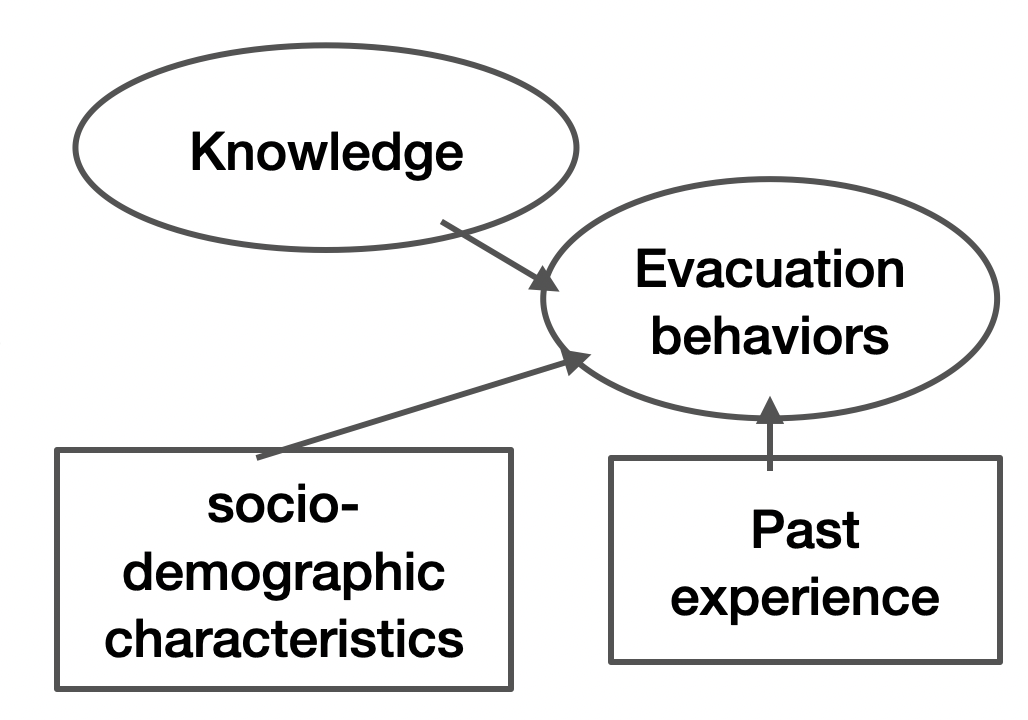
\includegraphics[width=0.5\linewidth]{Figure/Figure7.png}
  \centering
  \caption{Hypothesis base on previous research - 1 }
  \label{fig7}
\end{figure*}
%\fi

\begin{itemize}
\item Evacuation is significantly related to Socio-demographic factors, such as age, gender, etc, Socioeconomic factors, like educational attainment or household characteristics, etc, Personal characteristics, like hazard experience, knowledge, abilities/impairments, etc. Also, evacuees tend to make use of their familiarity with the surroundings based on their knowledge.~\cite{ref9}
\end{itemize}

Based on this study, we can construct a relationship that age, gender, hazard experience,  educational attainment, knowledge, abilities could relate to Evacuation Behaviors, shown in Figure~\ref{fig8}. 

\begin{figure*}[h]
  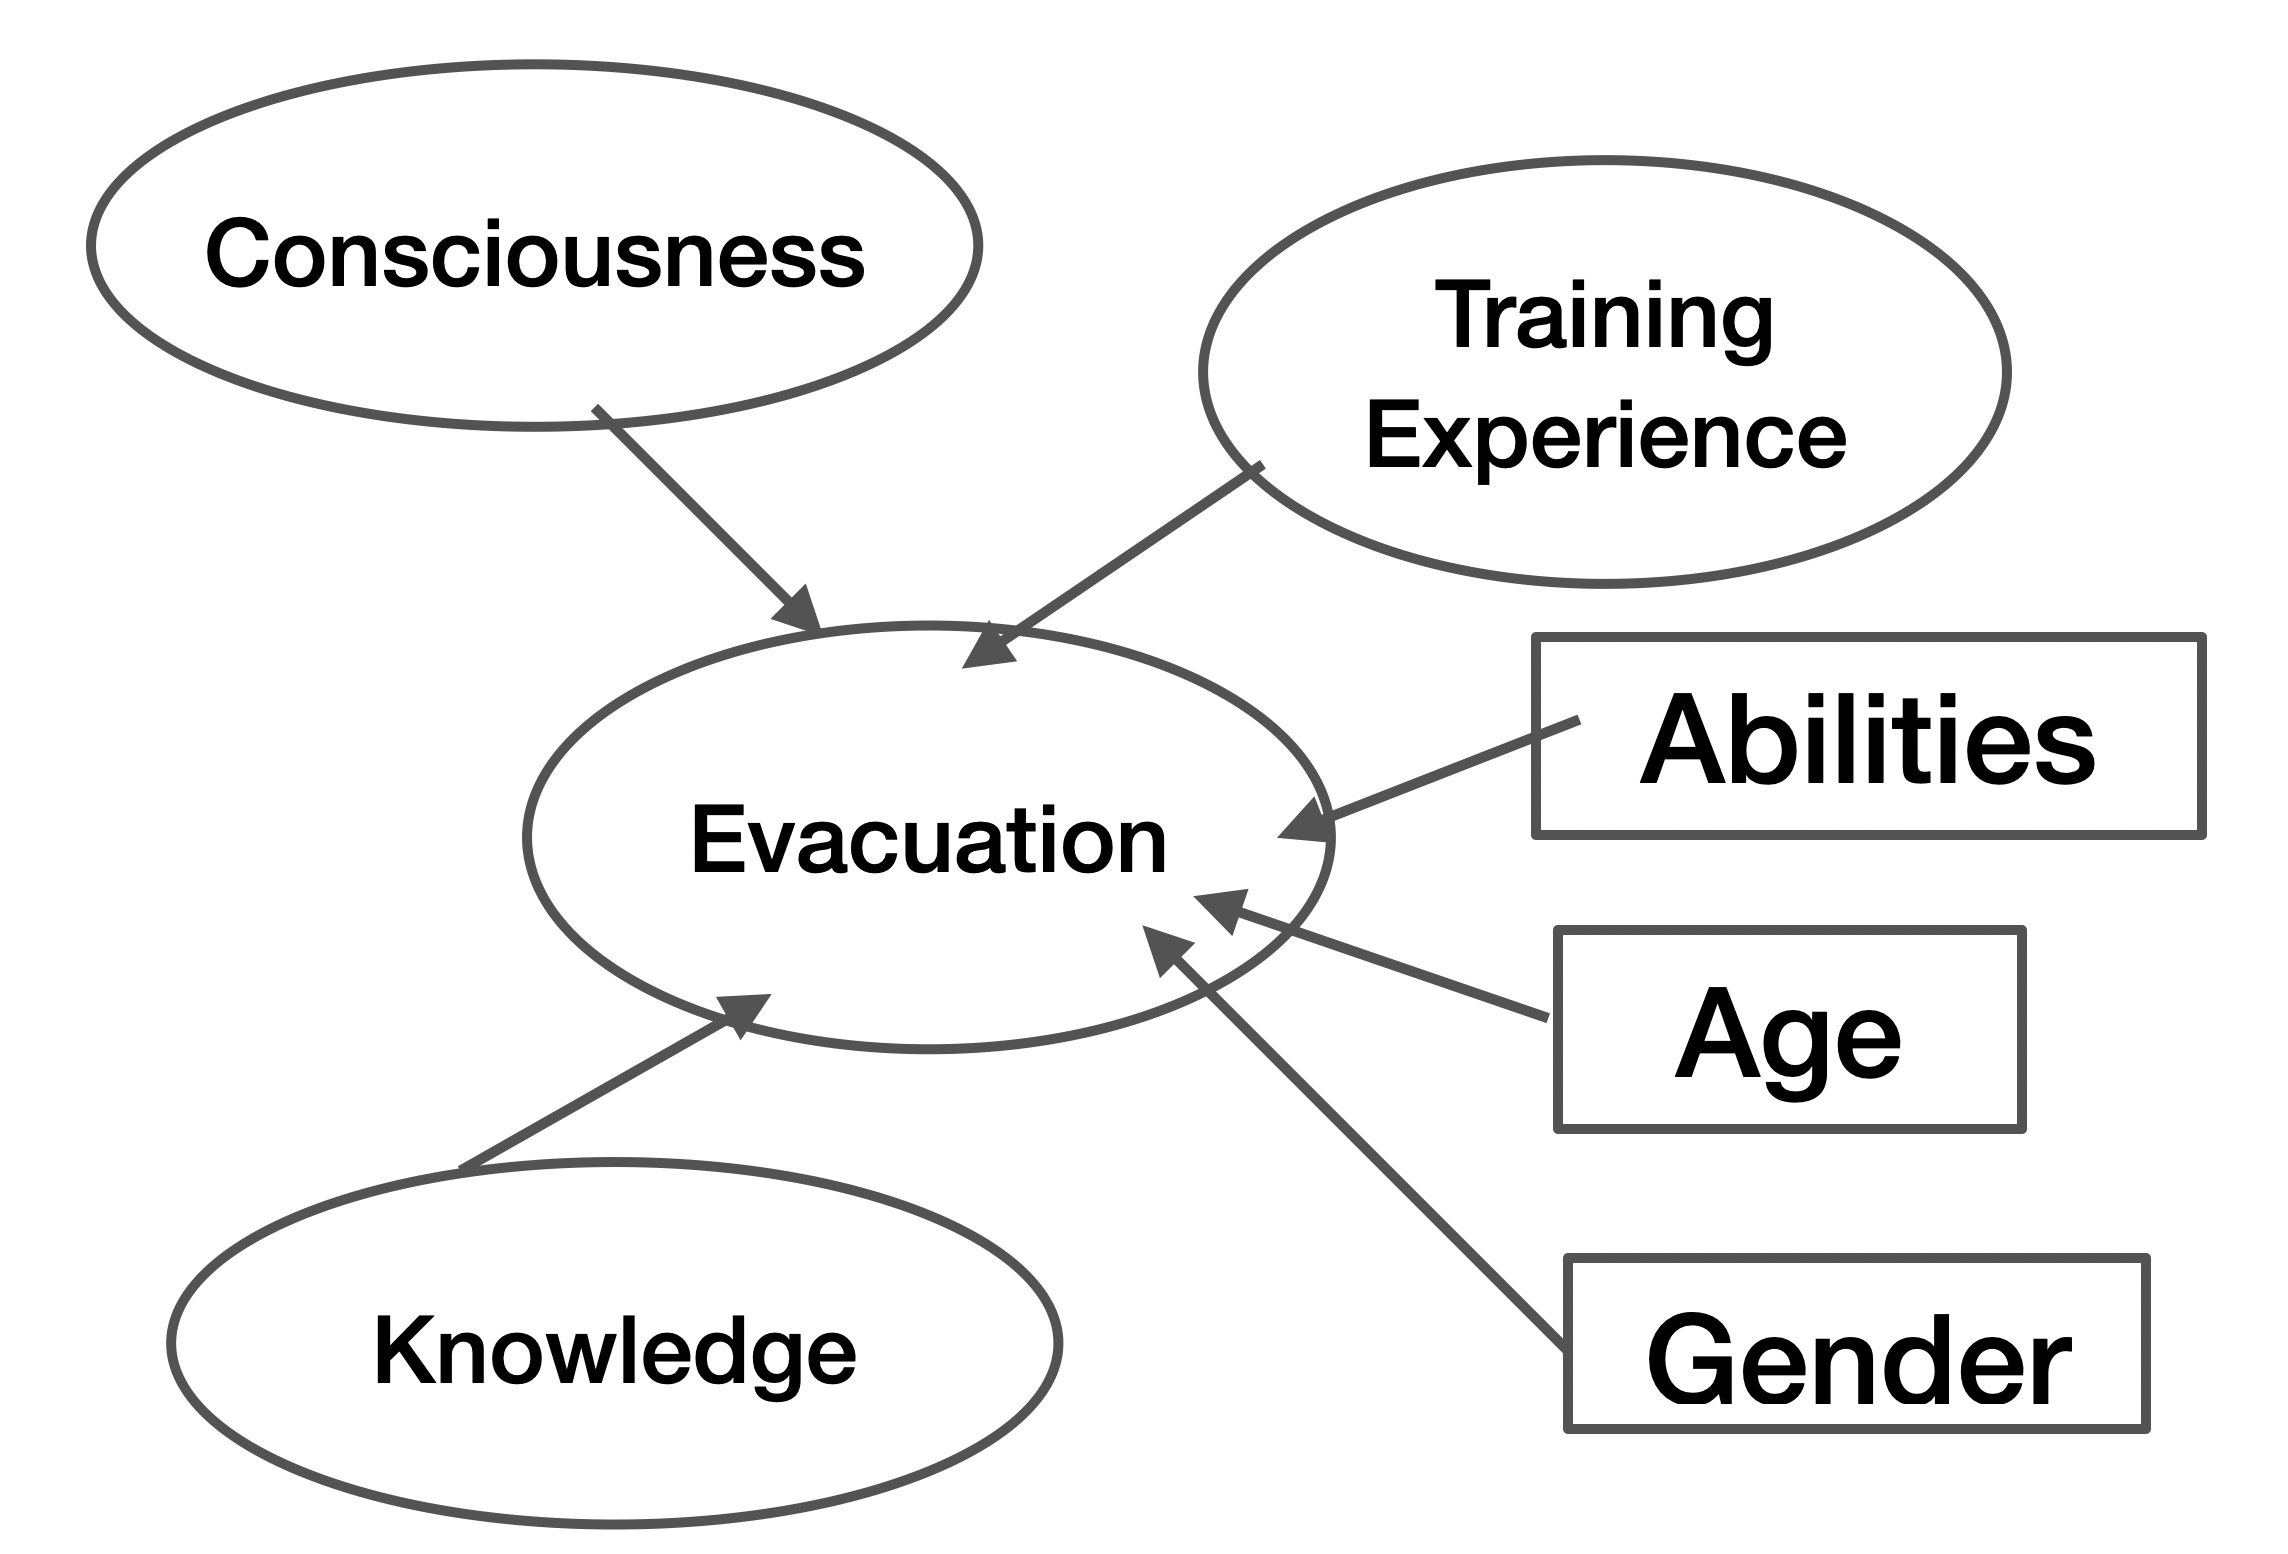
\includegraphics[width=0.5\linewidth]{Figure/Figure8.png}
  \centering
  \caption{Hypothesis base on previous research - 2 }
  \label{fig8}
\end{figure*}

In this study, we initially formulated three hypotheses (H1- H3 ) corresponding to the causal relationships between four latent variables based on the above results, which are shown in Figure~\ref{fig30}.

\begin{itemize}
\item[\textbf{H1}] Disaster Prevention Consciousness has a positive effect on respondents' attitudes toward Safety Tips.
\item[\textbf{H2}] Knowledge and Perception on earthquakes has a positive effect on respondents' attitudes toward Safety Tips.
\item[\textbf{H3}] Training Experience has a positive effect on respondents' attitudes toward Safety Tips.
\end{itemize}

%%%%%%%%%%%%%%%%%%%%%%%
%\iffalse
\begin{figure*}[h]
  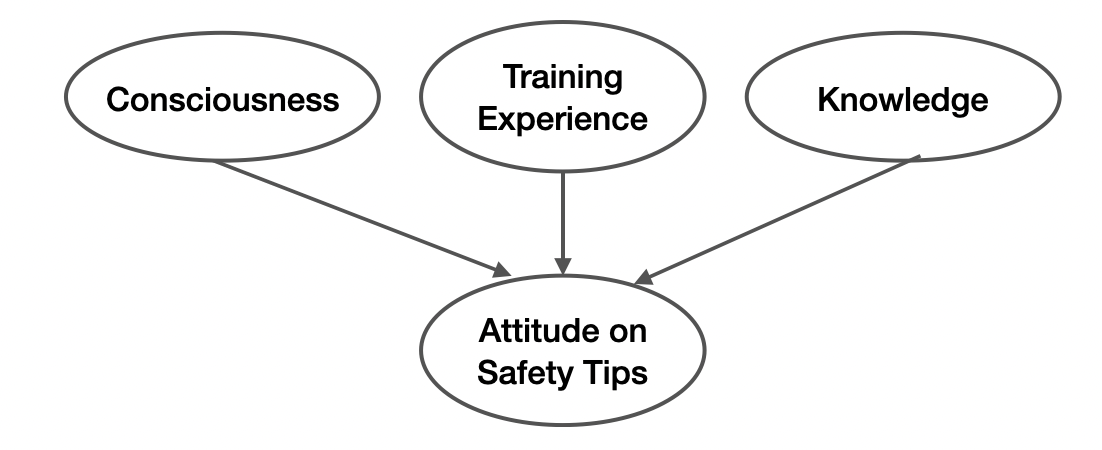
\includegraphics[width=0.5\linewidth]{Figure/Figure30.jpg}
  \centering
  \caption{Initial hypothesis used for SEM}
  \label{fig30}
\end{figure*}
%\fi

Each latent variable is represented by multiple indicators, and the summary statistics of these indicators are shown in Table~\ref{table5}. The latent variable 'Disaster Prevention Consciousness' has 5 manifest variables, which are disastrous imagination (Q1), sense of crisis (Q2), others-oriented type (Q3), anxiety (Q4), apathy about disasters (Q5). The latent variable 'Disaster Knowledge' has 2 manifest variables, which are knowledge about earthquakes (Q9) and knowledge of how to respond to a disaster (Q10). The latent variable 'Training Experience' has 2 manifest variables, which are the total score of earthquake/tsunami/typhoon/fire training experiences. (Q6) and the number of times participating in earthquake/tsunami/typhoon/fire disaster training (Q7). Latent variable 'Attitude toward Safety Tips' has 4 manifest variables, which are trust level (Q17\_1), the priority of use (Q17\_2), usefulness (Q17\_3), and the possibility of future use (Q17\_4). In addition to this, there are some directly observable manifest variables, such as demographic variables, etc. These variables will be involved in the SEM as manifest variables. Since it is uncertain whether these variables affect their attitude towards Safety Tips, a sample test will be conducted subsequently. There are 6 manifest variables, which are Age (FQ3), Gender (FQ2), number of visits to Japan within 1 year (FQ5), number of visits to any country in the world within 1 year (FQ4), Japanese level (FQ7), and the severity of the earthquake experienced (Q8). Therefore, the final Structural Equation Modeling shows in Figure~\ref{fig9}.

%%%%%%%%%%%%%%%%%%
%\iffalse
\begin{table}[h]
  \caption{Latent variables and manifest variables used for SEM. }
  \label{table5}
  \centering
  \begin{tabular}{|c|l|c|}
  \hline
  Latent variables &  \multicolumn{1}{c|}{Manifest Variables} &  \begin{tabular}{c}Number of\\variables\\included \end{tabular} \\
  \hline
  \multirow{5}{*}{\begin{tabular}{c}Disaster prevention\\consciousness \end{tabular}} & Disastrous Imagination (Q1) & 1\\
  \cline{2-3}
        & Sense of crisis (Q2) & 1 \\
  \cline{2-3}
        & Other-directed type (Q3) & 1\\
  \cline{2-3}
        & Anxiety (Q4) & 1\\
  \cline{2-3}
        & Apathy about disasters (Q5) & 1\\
  \hline
  \multirow{2}{*}{Disaster knowledge} & Knowledge about earthquakes (Q9) & 1\\
  \cline{2-3}
        & Knowledge of how to respond to a disaster (Q10) & 1\\
  \hline
  \multirow{2}{*}{Training experiences} & \begin{tabular}{l}Total score of earthquake/tsunami/typhoon/\\fire training experiences. (Q6)\end{tabular} & 4 \\
  \cline{2-3}
        & \begin{tabular}{l}Number of times participating earthquake/\\tsunami/typhoon/fire disaster training (Q7)\end{tabular} & 4\\
  \hline
   \multirow{4}{*}{\begin{tabular}{c}Attitude toward\\Safety Tips\end{tabular}} & Trust level & 1 \\
  \cline{2-3}
                                            & Priority of use & 1\\
  \cline{2-3}
                                            & Usefulness & 1 \\
  \cline{2-3}
                                            & Possibility of future use & 1 \\
  \hline
   / & Age & 1\\
  \hline
   / & Gender & 1\\
   \hline
   / & Number of visit Japan within 1 year & 1\\
   \hline
   / & \begin{tabular}{l}Number of visit any country in the world\\within 1 year\end{tabular} & 1 \\
   \hline
   / & Japanese level & 1 \\ 
   \hline
   / & The severity of the earthquake experienced & 1 \\
   \hline
  \end{tabular}
\end{table}
%\fi
%%%%%%%%%%%%%%%%%%%%%%%%%%%%%%%%
%\iffalse


\begin{figure*}[h]
  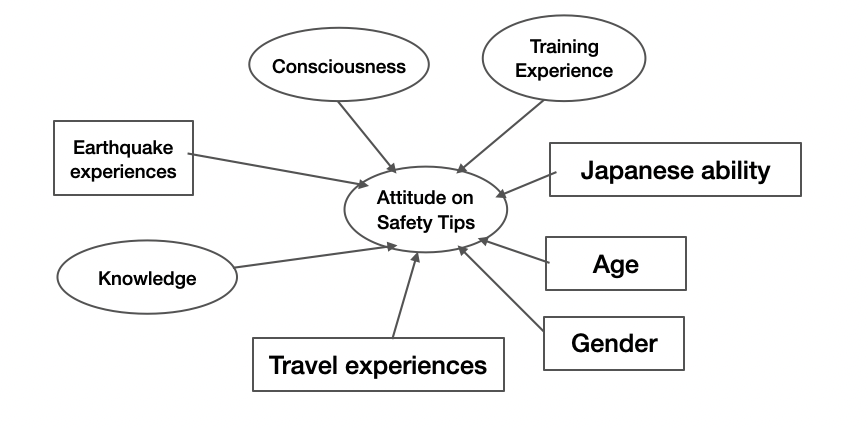
\includegraphics[width=\linewidth]{Figure/Figure9.png}
  \centering
  \caption{Conceptual model used for SEM }
  \label{fig9}
\end{figure*}


\subsection{Step 3. Define variables}
The third step is to define each variable. This part requires a definition of all the variables. The definitions of manifest variables are shown in Table~\ref{table2item2}, Table~\ref{table2item3}, Table~\ref{table2item4}, and Table~\ref{table2item6}, including Disaster Prevention Consciousness, Disaster Knowledge, Training experience, and Attitude toward Safety Tips. The definitions of manifest variables are shown in Table~\ref{table2item1} and  Table~\ref{table2item3}, including Age (FQ3), Gender (FQ2), number of visits to Japan within 1 year (FQ5), number of visits to any country in the world within 1 year (FQ4), Japanese level (FQ7), and the severity of the earthquake experienced (Q8).


\subsection{Step 4. Sample data collection and processing}
The data are offered by the Economic and Social Research Institute mentioned in Chapter~\ref{c3}, and the data processing methods are shown in the following. 

\begin{itemize}
\item Item 1 (FQ2-FQ5,FQ7)
\end{itemize}

FQ2: (Male) = 1; (Female) = 2;

FQ3: (Age\,Under\,15) = 1; (Age 16-19) = 2; (Age 20-29) = 3; (Age 30-39) = 4; (Age 40-49) = 5; (Age 50-59) = 6; (Age 60-69) = 7; (Age Over 70) = 8;

FQ4\&FQ5: (0 time) = 0; (1 time) = 1; (2 times) = 2; (3 to 4 times) = 3; (5 to 6 times) = 4; (7 to 9 times) = 5; (Over 10 times) =6;


FQ7: (Cannot understand) = 1; (Basic) = 2; (Intermediate) = 3; (Up Level) = 4; 

\begin{itemize}
\item Item 2 (Q1-Q5)
\end{itemize}

Since each of Q1-Q5 has four sub-problems. Here will use the mean values of the four sub-problems as the final data. For example, Q1 = $mean$ (Q1\_1, Q1\_2, Q1\_3, Q1\_4), Q2-Q5 are processed in the same way.

\begin{itemize}
\item Item 3 (Q6-Q8)
\end{itemize}

Q6 is about past disaster training participation experience. There are four types of disasters: Q6\_1 earthquake, Q6\_2 tsunami, Q6\_3 typhoon, and Q6\_4 fire. Each of them has 12 different types of training experience, shown as Q6\_1/2/3/4\_1 to Q6\_1/2/3/4\_12. Respondents answered with 'Yes' or 'No' in these questions. If none of them were experienced before, 'Yes' was selected in Q6\_1/2/3/4\_13 to indicate that the respondent did not have any of the 12 experiences mentioned above. 

Therefore, 

Q6\_1 = $sum$ (Q6\_1\_1 + Q6\_1\_2 +\dots+ Q6\_1\_12);

Q6\_2 = $sum$ (Q6\_2\_1 + Q6\_2\_2 +\dots+ Q6\_2\_12);

Q6\_3 = $sum$ (Q6\_3\_1 + Q6\_3\_2 +\dots+ Q6\_3\_12);

Q6\_4 = $sum$ (Q6\_4\_1 + Q6\_4\_2 +\dots+ Q6\_4\_12).

Q7 is times of past disaster training experiences. There are also four types of disasters: Q7\_1 earthquake, Q7\_2 tsunami, Q7\_3 typhoon, and Q7\_4 fire.
 
(one time) = 1; (2-3 times) = 2; (4-6 times) = 3; (Over 7 times) =4;

Q8 is about the severity of the earthquake experienced.

(MMI intensity 5 or less / intensity 3 or less) = 1; (MMI intensity 6 / intensity 4) = 2; (MMI intensity 7 / intensity 5 weak) = 3; (MMI intensity 8 / intensity 5 strong) = 4; (MMI intensity 9 / intensity 6 weak) = 5; (MMI intensity 10 / intensity 6 strong) = 6; (MMI intensity 11 to 12 / intensity 7) = 7; (no experience) = 0.


\begin{itemize}
\item Item 4 (Q9-Q10)
\end{itemize}

Q9 has six sub-problems, Q10 has nine sub-problems. Here will use the mean values of the sub-problems as the final data. 

Therefore, 

Q9 = $mean$ (Q9\_1, Q9\_2, \dots, Q9\_6);

Q10 = $mean$ (Q10\_1, Q10\_2, \dots, Q10\_9).

\begin{itemize}
\item Item 6 (Q15-Q17)
\end{itemize}

Q15: (Don't know) = 1; (Only heard name before) = 2; (Know exactly) = 3;

Q16: (Never used before) = 0; (Used before) = 1;
 
Q17\_1, Q17\_2, Q17\_3, Q17\_4: use original data.

\subsection{Step 5. Reliability and validity testing (EFA/CFA)}
\label{step5}
The first measurement theory that we need to understand in Structural Equation Modeling is that the observed values equal true values plus bias and noise. Reliability means the degree to which the results are consistent when the same method is used to measure the same object repeatedly. As a result, Reliability indicates how much the measure is free from random error (noise). Reliability is the consistency, stability, and reliability of test results, and is generally expressed in terms of the internal consistency of the test. The higher the reliability coefficient, the more consistent, stable, and reliable the test results are. In addition, the systematic error has little effect on reliability in Reliability tests. Because systematic errors always affect the measurement values, in the same way, they do not cause inconsistency. On the contrary, random errors may cause inconsistency and thus reduce the difficulty. Reliability will be tested through the evaluation of Cronbach's alpha value by SPSS. 

Validity refers to the degree to which a measurement tool or instrument can accurately measure what is to be measured. As a result, Validity indicates how much the measure is free from systematic error (bias). Validity means that the results measured reflect what is intended to be measured and that the results measured are what was intended to be measured. Validity is an indicator of the degree of validity of a measurement instrument, i.e., the degree to which the instrument can measure the characteristics to be measured, and can be simply interpreted as the accuracy and usefulness of a test. 

There are two types of Validity Analysis, one is Exploratory Factor Analysis (EFA), which is generally used in SPSS. EFA is measured through dimensionality reduction. For example, if the questionnaire has 100 questions, then how many dimensions these 100 questions should be grouped into can be achieved by EFA. But most self-designed questionnaires, in fact, when designing the questionnaire, there is already a potential dimensional division. The other one is Confirmatory Factor Analysis (CFA). Compared with EFA, CFA can be used to check the compliance of the three types of validity, including the compliance of the model fit, the consistency of the indicators within each dimension, and the differentiation of the indicators from external indicators. CFA estimates latent variables based on correlated changes in the dataset, which can reduce data dimensionality, standardize the size of multiple metrics, and account for correlations inherent in the dataset~\cite{ref16}. CFA is generally used by Amos, and it is measured by Construct Validity, Convergent Validity, and Discriminant Validity. The main purpose of Construct Validity is to check the fitness of the whole model. If the fit is low, the model, the latent variables, and the relationships between the latent variables are adjusted to improve the fit. The adjustments are explained in subsection~\ref{s7}. 

The Convergent Validity looks at the strength of the correlation between several topics within the same dimension. 
Regarding Convergent Validity, it is used to assess the internal consistency of several items and has similarity with Cronbach's alpha. However, when there are multiple dimensions of the scale, it is not appropriate to use Cronbach's alpha to calculate its internal consistency reliability~\cite{ref29,ref30}. Convergent Validity is generally assessed using Composite Reliability (CR) and Average of Variance Extracted (AVE) to assess Convergent Validity. Convergent Validity~\cite{ref33} is estimated by the standardized factor loading and the respective error variance, the equation shown in the following Formula~\ref{for2}. $\lambda$ denotes the standardized factor loading for item $i$ and $\epsilon$ denotes the respective error variance for item $i$. The error variance is estimated based on the value of the standardized loading ($\lambda$) as Formula~\ref{for3}. And the R-square value is the percent of the variance, which is explained by the latent variable. It is estimated based on the value of the standardized loading ($\lambda$) as Formula~\ref{for4}. In this study, we will calculate CR value by Composite Reliability Calculator~\footnote{https://www.thestatisticalmind.com/composite-reliability/}. Higher CR indicates higher internal consistency and convergence of the conformation. The commonly used evaluation criterion in research is the one mentioned in the book Multivariate data analysis. 5th Edition~\cite{ref32}, that is CR value above 0.7 is acceptable. However, Fornell and Larcker (1981)~\cite{ref31} also suggested that a CR value above 0.6 is acceptable. 

\begin{equation}
\label{for2}
CR=\frac{(\sum \lambda_i )^2}{(\sum \lambda_i )^2+(\sum \epsilon _i )}
\end{equation}

\begin{equation}
\label{for3}
\epsilon_i = 1-\lambda_i^2  
\end{equation}

\begin{equation}
\label{for4}
r^2 = \lambda_i^2 = 1- \epsilon_i  
\end{equation}

Regarding AVE, AVE refers to the average of the explanatory power of the latent variables on the observed variables, and the equation is shown in the following Formula~\ref{for5}~\footnote{https://en.wikipedia.org/wiki/Average\_variance\_extracted}. Here, $k$ is the number of items, $\lambda_i$ is the factor loading of item $i$, and the $Var(e_i)$ is the variance of the error of item $i$. The higher the AVE, the higher the Convergent Validity. According to Fornell and Larcker (1981)~\cite{ref31}, the AVE value needs to be greater than 0.5. Squared Multiple Correlation (SMC) and Std. Factor Loading is used in the calculation of CR and AVE. A higher SMC indicates a higher proportion of true scores and can be used to calculate the confidence level.

\begin{equation}
\label{for5}
AVE = \frac{\sum_{i=1}^{k} \lambda_i^2 }{\sum_{i=1}^{k} \lambda_i^2+\sum_{i=1}^{k} Var(e_i)}
\end{equation}

Convergent Validity and Discriminant Validity can be viewed relatively. The Discriminant Validity is to see whether the differentiation between different dimensions and between topics meets the standard. There are three ways to achieve Discriminant Validity in CFA. The first is to compare the correlation coefficients of the two latent variables, and if their 95\% confidence intervals cover 1.00, it indicates that the constructs lack discriminant power. The second one is to compare two CFA models, one model is a validity model, and the other sets the correlation coefficient of the two potential variables to 1. That is, the fully correlated model/single-factor model. Theoretically, the latter will have a lower fit. If the former is significantly better than the latter, the discriminative power of the area between the two constructs is qualified. If the former is not significantly better than the latter, it means that the two constructs lack zone discrimination~\cite{ref34,ref35}. The third comparison was made using AVE to compare whether the mean AVE of two latent variables was greater than the squared correlation coefficient of the two latent variables~\cite{ref31}. The third method was adopted in this study. Because the questionnaire used in this study has a clear division of dimensions, EFA is not required for this study, and the results of Reliability Analysis and CFA will be presented in Chapter~\ref{c5}.


\subsection{Step 6. Model Fit Test}
\label{step6}
Model Fit Test is primarily used for the CFA's Construct Validity test. The fit indices of the single-path coefficient test, which are the p-values and standard errors, and the overall model fit, which are the $\chi^2$ and RMSEA values, are used to evaluate the SEM~\cite{ref16}.

\begin{itemize}
\item \textbf{Chi-square Test ($\chi^2$):} It investigates the possibility of a discrepancy between the model-implied covariance matrix and the original covariance matrix. As a result, the non-significant difference is preferred. The Chi-square test should not be taken too seriously~\cite{ref22,ref23,ref24}, because it is very sensitive to sample size and is not comparable across different SEMs. CMIN/DF is the minimum variance divided by its degrees of freedom. To reduce the effect of sample size, the chi-squared value is adjusted by the degrees of freedom~\cite{ref41}. In prior studies such as Wheaton et al. (1977)~\cite{ref24} the authors suggest that the CMIN/DF should be calculated as a measure of goodness of fit. However, one problem with the CMIN/DF value is that it is a difficult value to clearly define a critical criterion. Carmines and McIver (1981)~\cite{ref36} suggests a CMIN/DF of 2:1 or 3:1. Ullman (2001)~\cite{ref37} considered that within 2 is called a good model fit. Kline (2005)~\cite{ref38} suggested that within 3 is acceptable. Schumacker and Lomax (2004)~\cite{ref39} suggest a more lenient fit around 5 or less. Hair et al., 1998~\cite{ref40}indicated that the smaller the ratio of cardinality to degrees of freedom, the better the fit of the model. The value should preferably be less than 3, but not less than 1.
\item \textbf{Root Mean Square Error of Approximation (RMSEA):}  RMSEA indicates badness of fit, which is a common evaluation value for SEM. The RMSEA value of 0 means perfect fit, a higher value means short of fit~\cite{ref25}. RMSEA could be less sensitive to sample size than the Chi-square test, so RMSEA can be more useful when detecting model misspecification. McDonald \& Ho~\cite{ref2} verified RMSEA should be less than 0.08. Takahiro HOSHINO~\cite{SEMres} summarized a broader range of evaluation value, it mentioned that if RMSEA< 0.05 means 'close fit'; if RMSEA $< 0.08$ means 'fair fit'; if RMSEA$< 0.01$ means 'moderate fit'; if RMSEA over 0.01means the model is not good~\cite{ref3,ref4,ref5}. 
\item \textbf{Comparative Fit Index (CFI):} The amount of variance accounted for in a covariance matrix is represented by the CFI. Its value ranges from 0.0 to 1.0. A higher CFI value indicates a more accurate model fit. Bentler~\cite{ref6} verified that a CFI value close to 1 indicates a very good fit. Traditionally, a CFI of 0.9 or higher is considered a good match~\cite{ref43,ref44}. Compared with the Chi-square test, CFI can be less sensitive to sample size~\cite{ref26}.
\end{itemize}

In general, the more fit indices that are applied to SEM, the more likely it is that a misspecified model will be rejected, and the less likely it is that a good model will be rejected. As a result, the study must employ at least two distinct fit indices~\cite{ref17}. Some indices have recommended cutoff values, but no indices can be utilized as the standard for all applications~\cite{ref18,ref19,ref20,ref21}. Fan (2016)~\cite{ref16} mentioned other types of evaluation values for model fit, but this study decided to use the common evaluation values that were detailed mentioned above. 

\subsection{Step 7. Model adjustment and modification}
\label{s7}
Based on the structural validity results discussed earlier, the next step is to revise and adjust the Structural Equation Modeling. Therefore, the core of model revision and adjustment is to revise and optimize the measurement model for each latent variable to ensure that the overall model fitness is up to standard. The method of optimizing the measurement model, in addition to removing the less significant variables through the reliability results of SPSS, is to modify the indicator correction suggestions through the output of Amos. In general, there are two indicators. The first one is the Standardized Regression Weights (SRW), or Squared Multiple Correlation (SMC), which is the square of the SRW, and the SRW should be greater than 0.7 and the SMC should be greater than 0.5. Following is the common acceptable range for SRW/SMC. SRW$ \geq 0.95$ indicates that there is a problem with the framing of the conformation (the reason will be explained in ~\ref{step 8}; SRW$ \geq 0.63$ means SMC is greater than 40\%, proving very good; SRW$\geq0.55$ represents SMC greater than 30\%, proving good; SRW$ \geq0.45$ represents SMC greater than 20\%, proving more ordinary; SRW$\geq0.32$ means SMC is greater than 10\%, which proves to be poor; SRW$< 0.32$, means the model fails for the test~\cite{ref15,ref27}. 

Another one is the Modification Indices. By M.I. value of covariances in the modification indices results. M.I. value refers to the amount of change that can be reduced by the corrected chi-square value, and the higher the value, the more it helps to correct the model. However, because the correlation between residuals is not academically interpretable. This is because the premise assumptions state that the residuals are independent. Therefore, correcting the model is done by removing the problem itself where the residuals have the greatest impact. As mentioned before, since the survey used in this study has a clear dimensional division, EFA was not performed. Therefore, this part of the model fitness adjustment will be performed with the first method as the main one.


\subsection{Step 8. Path coefficient analysis}
\label{step8}
First look at Unstandardized Estimates, which describes how many units the dependent variable increases for each unit increase in the independent variable. Before evaluating the SEM fit, the estimated coefficients must be checked by Offending estimates to determine whether they are outside the acceptable range. Specifically, the first should look at the estimated coefficients of the error terms, which should not be negative. Secondly, we have to look at the factor loadings and whether the path coefficients are significant. Next, we look at the Standardized Estimates, which describes how many standard deviations the dependent variable will increase for each standard deviation increase in the independent variable. The factor loading of the measurement model should be greater than 0.7 and the SMC greater than 0.5, which proves to be very good; However, in general, the factor loading of the scales developed by social science researchers is not too high considering that it may be limited by the nature of the measurement (e.g., the range of attitude measurement is too wide and not easily focused, the construct is too vague and not easily defined), the external interference and measurement error, or even the nature of the construct. Tabachnica and Fidell, (2007)~\cite{ref26} suggest that a factor loading of 0.55 or higher and an SMC of 0.3 or higher can be declared good. As for the structural model of SMC, the main focus on significance is sufficient. To summarize, Unstandardized Estimates are used to see if they are significant, and Standardized Estimates are used to see the magnitude of the influence factors.


\subsection{Step 9. Hypothesis testing and conclusion analysis}
The hypothesis testing and conclusion analysis section is equivalent to a summary of SEM. We need to describe in detail the SEM model, the results of the model fitness, and the significance of the hypothesis relationships. The results are used to summarize the similarities/differences between the original hypothesis of the study and the results given by SEM, and to give an analysis based on the results. Finally, it is considered that this study needs to propose some suggestions for the future development of Safety Tips, so a proposal will be presented based on the conclusions presented in the results.



\section{Result}
The results of the statistical description with the maximum value, minimum value, mean, and standard deviation for each variable are shown in Table~\ref{table27}.

\begin{table}[h]
  \caption[Statistical Description]{Statistical Description (N=491)}
  \label{table27}
  \centering
  \begin{tabular}{l|cccc}
 \hline
\multicolumn{1}{c|}{Variable} & Min value  & Max value & Mean & Standard Deviation \\
 \hline
Country	& 2&6&4.32&1.30\\
gender&1&2&1.48&0.50\\
age&2&7&4.37&1.26\\
Visit\_country&1&10&4.39&2.61\\
Visit\_Japan&1&11&4.99&2.92\\
Japanese\_Level&1&4&2.59&0.77\\
Q1\_disastrous\_imagination&1&6&4.94&1.02\\
Q2\_ sense\_of\_crisis&1&6&4.95&1.01\\
Q3\_others-oriented\_type&1&6&5.08&0.99\\
Q4\_anxiety&1&6&4.55&1.03\\
Q5\_ apathy\_about\_disasters&1&6&3.83&1.41\\
Q6\_1\_earthquake&0&12&4.95&3.74\\
Q6\_2\_tsunami&0&12&4.53&3.33\\
Q6\_3\_typhoon&0&12&4.6&3.43\\
Q6\_4\_fire&0&12&5.01&4.06\\
Q7\_1\_earthquake&0&4&1.66&1.60\\
Q7\_2\_tsunami&0&4&0.80&1.27\\
Q7\_3\_typhoon&0&4&0.72&1.29\\
Q7\_4\_fire&0&4&1.48&1.61\\
Q8\_experience\_earthquake&1&8&3.15& 1.87\\
Q9\_knowledge\_earthquake&1&6&4.88&0.97\\
Q10\_knowledge\_response&1&6&5.01&0.95\\
Q15\_Safetytips\_awareness&2&3&2.73&0.45\\
Q16\_Safetytips\_usage&1&1&1&0\\
Q17\_Safetytips\_trust&1&6&4.8&1.31\\
Q17\_Safetytips\_priority&1&6&4.95&1.08\\
Q17\_Safetytips\_usefulness&1&6&5.10&1.01\\
Q17\_Safetytips\_future\_use&1&6&5.11&1.02\\
 \hline
  \end{tabular}
\end{table}

For some group-based data, the frequency descriptions of these variables are shown in the following. The frequency description of Item 1, including Country, Gender, Age, number of visited countries, number of visited Japan, Japanese Level are shown in \crefrange{table28a}{table28f}. Table~\ref{table28g} is the frequency description of Item 3, that is the severity of the earthquake experience.

\begin{table}[h]
  \caption[Frequency Description of Country]{Frequency Description of Country (N=491)}
  \label{table28a}
  \centering
  \begin{tabular}{l|cc}
 \hline
\multicolumn{1}{c|}{Category}&Number&Rate\\
 \hline
China&78&15.90\%\\
South Korea&42&8.60\%\\
Thailand&105&21.40\%\\
Indonesia&179&36.50\%\\
the UK&87&17.70\%\\
 \hline
  \end{tabular}
\end{table}

\begin{table}[h]
  \caption[Frequency Description of Gender]{Frequency Description of Gender (N=491)}
  \label{table28b}
  \centering
  \begin{tabular}{l|cc}
 \hline
\multicolumn{1}{c|}{Category}&Number&Rate\\
 \hline
Male   & 253 & 51.50\% \\
Female & 238 & 48.50\% \\
 \hline
  \end{tabular}
\end{table}

\begin{table}[h]
  \caption[Frequency Description of Age]{Frequency Description of Age (N=491)}
  \label{table28c}
  \centering
  \begin{tabular}{l|cc}
 \hline
\multicolumn{1}{c|}{Category}&Number&Rate\\
 \hline
Age 16-19   & 13  & 2.60\%  \\
Age 20-29   & 136 & 27.70\% \\
Age 30-39   & 126 & 25.70\% \\
Age 40-49   & 113 & 23\%    \\
Age 50-59   & 77  & 15.70\% \\
Age 60-69   & 26  & 5.30\%  \\
Age over 70 & 0   & 0\% \\
 \hline
  \end{tabular}
\end{table}

\begin{table}[h]
  \caption[Frequency Description of number of visited country ]{Frequency Description of number of visited country (N=491)}
  \label{table28d}
  \centering
  \begin{tabular}{l|cc}
 \hline
\multicolumn{1}{c|}{Category}&Number&Rate\\
 \hline
0 time        & 0                    & 0\%                  \\
1 time        & 73                   & 14.90\%              \\
2 times       & 63                   & 12.80\%              \\
3 to 4 times  & 152                  & 31\%                 \\
5 to 6 times  & 95                   & 19.30\%              \\
7 to 9 times  & 99                   & 20.20\%              \\
Over 10 times & 9                    & 1.80\%               \\
 \hline
  \end{tabular}
\end{table}

\begin{table}[h]
  \caption[Frequency Description of number of visited Japan]{Frequency Description of number of visited Japan (N=491)}
  \label{table28e}
  \centering
  \begin{tabular}{l|cc}
 \hline
\multicolumn{1}{c|}{Category}&Number&Rate\\
 \hline
0 time        & 0   & 0\%     \\
1 time        & 47  & 9.60\%  \\
2 times       & 65  & 13.20\% \\
3 to 4 times  & 147 & 29.90\% \\
5 to 6 times  & 85  & 17.30\% \\
7 to 9 times  & 81  & 16.50\% \\
Over 10 times & 66  & 13.40\% \\
 \hline
  \end{tabular}
\end{table}

\begin{table}[h]
  \caption[Frequency Description of Japanese Level]{Frequency Description of Japanese Level (N=491)}
  \label{table28f}
  \centering
  \begin{tabular}{l|cc}
 \hline
\multicolumn{1}{c|}{Category}&Number&Rate\\
 \hline
Cannot understand                    & 25  & 5.10\%  \\
Basic        & 214 & 43.60\% \\
Intermediate & 190 & 38.70\% \\
Up level     & 62  & 12.60\% \\
 \hline
  \end{tabular}
\end{table}

\begin{table}[h]
  \caption[Frequency Description of severity of the earthquake experienced]{Frequency Description of severity of the earthquake experienced (N=491)}
  \label{table28g}
  \centering
  \begin{tabular}{l|cc}
 \hline
\multicolumn{1}{c|}{Category}&Number&Rate\\
 \hline
MMI intensity 5 or less / intensity 3 or less & 110 & 22.40\% \\
MMI intensity 6 / intensity 4                 & 90  & 18.30\% \\
MMI intensity 7 / intensity 5 weak            & 119 & 24.20\% \\
MMI intensity 8 / intensity 5 strong          & 80  & 16.30\% \\
MMI intensity 9 / intensity 6 weak            & 30  & 6.10\%  \\
MMI intensity 10 / intensity 6 strong                                 & 18  & 3.70\%  \\
MMI intensity 11 to 12 / intensity 7                                  & 30  & 6.10\%  \\
no earthquake experience                                              & 14  & 2.90\%  \\
 \hline
  \end{tabular}
\end{table}

Since the results in section~\ref{task3}, the differences in gender and severity of experienced earthquakes did not show a significant effect in the responses of Attitude toward Safety Tips. This also means that these two manifest variables would not need to be considered in SEM. Therefore, the four manifest variables used in the SEM were age, number of visited countries, number of visited Japan, and Japanese level. Among them, only the ANOVA results of the manifest variables number of visited Japan and Japanese level showed that the differences were significant for all four attitude related questions. The results of age, the number of visited countries, and other manifest variables only show that the differences are significant for some of the questions, not for all of them. However, since the results cannot be deleted directly, after all, there are some questions with good significance test results, so they are still retained in the SEM.

\subsection{Test for latent variables }
The results of the correlation test of three latent variables which are Disaster prevention consciousness, Training experience, Knowledge, and perception of earthquakes are presented in Table~\ref{table33}. As ** means significant correlation at $p<0.01$ level, so from the results we can know that there are significant correlations between Disaster prevention consciousness and Knowledge and perception on earthquakes, also Knowledge and perception on earthquakes and Training experience.

\begin{table}[h]
  \caption{Correlation test result of latent variables}
  \label{table33}
  \centering
\begin{tabular}{c|ccc}
\hline
         & Consciousness & Knowledge & Training\_Experience \\
\hline
Consciousness        & 1             &           &                     \\
Knowledge            & .669**        & 1         &                     \\
Training\_Experience   & 0.056         & .352**    & 1            \\
\hline
\multicolumn{4}{l}{** means significant correlation at $p<0.01$.}
\end{tabular}
\end{table}


\subsection{Reliability }



The survey selected for this study contained three sets of questions, which are Disaster Prevention Consciousness, Knowledge and Perception on earthquakes, and Attitude toward Safety Tips. Disaster Prevention Consciousness contains 5 sub-problems with a total of 20 questions. Knowledge and Perception on earthquakes contain 2 sub-questions with a total of 15 items. Attitude toward Safety Tips contains 4 sub-questions with a total of 4 items. In order to ensure the internal consistency of the scale, it is necessary to pass the reliability test first before conducting CFA. The internal consistency was tested by calculating the internal consistency reliability coefficient Cronbach's alpha value of the scale. When multiple questions are asked about a characteristic and the sum of the responses (scale scores) is used as the characteristic scale, the reliability coefficient that assesses whether each questionnaire item (variable) measures the same concept or object as a whole (internal consistency) is called Cronbach's alpha. Cronbach's alpha is calculated by the following Formula~\ref{for1}.

\begin{equation}
\label{for1}
\alpha = \frac{m}{m-1} \left(1 - \frac{\displaystyle \sum_{i = 1}^m{{\sigma_i}^2}}{{\sigma_x}^2} \right)
\end{equation}

$m$ means the number of items in the question; ${\sigma_i}^2$ means the variance of each question item; ${\sigma_x}^2$ means the variance of the total scale score for each question item. Cronbach's alpha has a value between 0 and 1, and the closer the value is to 1, the more reliable it is. The evaluation of Cronbach's alpha is shown in Figure~\ref{fig24}, as suggested by George and Mallery (2003).~\cite{ref1}. Cronbach's alpha  Cronbach's alpha of 0.9 indicates excellent internal consistency, 0.8 indicates good, 0.7 indicates acceptable, 0.6 indicates poor, and 0.5 unacceptable. The results of the reliability test are shown in Table~\ref{table34}, the Cronbach's alpha values of Disaster Prevention Consciousness is 0.902, for Knowledge and Perception on earthquakes is 0.952, and for Attitude toward Safety Tips is 0.875. The total Cronbach's alpha value for all above is 0.955. We can find that the Cronbach's alpha value of any one of them is satisfying the evaluation criteria.




\begin{table}[h]
  \caption[Reliability test]{Reliability test (N=491)}
  \label{table34}
  \centering
\begin{tabular}{c|c|cc|c|c}
\hline
 \multicolumn{2}{c}{}           & Question & \multicolumn{1}{c}{Mean}      & \multicolumn{1}{c}{Object number}         & \begin{tabular}{c}Cronbach's\\alpha value\end{tabular}   \\
\hline
                                                           &                                                             & Q1\_1    & 4.89$\pm$1.21 &                       &                          \\
                                                           &                                                             & Q1\_2    & 4.94$\pm$1.10  &                       &                          \\
                                                           &                                                             & Q1\_3    & 4.99$\pm$1.14 &                       &                          \\
                                                           & \multirow{-4}{*}{\begin{tabular}{c}Disastrous\\Imagination\end{tabular}}                    & Q1\_4    & 4.94$\pm$1.18 &                       &                          \\
\cline{2-4}
                                                           &                                                             & Q2\_1    & 4.85$\pm$1.29 &                       &                          \\
                                                           &                                                             & Q2\_2    & 4.96$\pm$1.21 &                       &                          \\
                                                           &                                                             & Q2\_3    & 4.93$\pm$1.19 &                       &                          \\
                                                           & \multirow{-4}{*}{\begin{tabular}{c}Sense of\\crisis\end{tabular}}                           & Q2\_4    & 5.07$\pm$1.12 &                       &                          \\
\cline{2-4}
                                                           &                                                             & Q3\_1    & 5.12$\pm$1.11 &                       &                          \\
                                                           &                                                             & Q3\_2    & 4.97$\pm$1.20  &                       &                          \\
                                                           &                                                             & Q3\_3    & 5.13$\pm$1.11 &                       &                          \\
                                                           & \multirow{-4}{*}{\begin{tabular}{c}Other-directed\\type\end{tabular}}                       & Q3\_4    & 5.11$\pm$1.09 &                       &                          \\
\cline{2-4}
                                                           &                                                             & Q4\_1    & 4.05$\pm$1.59 &                       &                          \\
                                                           &                                                             & Q4\_2    & 4.25$\pm$1.52 &                       &                          \\
                                                           &                                                             & Q4\_3    & 4.87$\pm$1.19 &                       &                          \\
                                                           & \multirow{-4}{*}{Anxiety}                                   & Q4\_4    & 5.04$\pm$1.11 &                       &                          \\
\cline{2-4}
                                                           &                                                             & Q5\_1    & 3.81$\pm$1.73 &                       &                          \\
                                                           &                                                             & Q5\_2    & 4.00$\pm$1.55  &                       &                          \\
                                                           &                                                             & Q5\_3    & 3.59$\pm$1.66 &                       &                          \\
\multirow{-20}{*}{\begin{tabular}{c}Disaster\\Prevention\\Consciousness\end{tabular}}       & \multirow{-4}{*}{\begin{tabular}{c}Apathy about\\disasters\end{tabular}}                    & Q5\_4    & 3.92$\pm$1.63 & \multirow{-20}{*}{20} & \multirow{-20}{*}{0.902} \\
\hline
                                                           &                                                             & Q9\_1    & 4.85$\pm$1.29 &                       &                          \\
                                                           &                                                             & Q9\_2    & 4.88$\pm$1.12 &                       &                          \\
                                                           &                                                             & Q9\_3    & 4.90$\pm$1.12  &                       &                          \\
                                                           &                                                             & Q9\_4    & 4.87$\pm$1.10  &                       &                          \\
                                                           &                                                             & Q9\_5    & 4.82$\pm$1.15 &                       &                          \\
                                                           & \multirow{-6}{*}{\begin{tabular}{c}Knowledge\\about\\earthquakes\end{tabular}}               & Q9\_6    & 4.94$\pm$1.11 &                       &                          \\
\cline{2-4}
                                                           &                                                             & Q10\_1   & 5.03$\pm$1.27 &                       &                          \\
                                                           &                                                             & Q10\_2   & 4.86$\pm$1.22 &                       &                          \\
                                                           &                                                             & Q10\_3   & 4.97$\pm$1.15 &                       &                          \\
                                                           &                                                             & Q10\_4   & 5.05$\pm$1.08 &                       &                          \\
                                                           &                                                             & Q10\_5   & 5.05$\pm$1.09 &                       &                          \\
                                                           &                                                             & Q10\_6   & 5.01$\pm$1.12 &                       &                          \\
                                                           &                                                             & Q10\_7   & 4.98$\pm$1.12 &                       &                          \\
                                                           &                                                             & Q10\_8   & 5.15$\pm$1.02 &                       &                          \\
\multirow{-15}{*}{\begin{tabular}{c}Knowledge and\\Perception on\\earthquakes\end{tabular}} & \multirow{-9}{*}{\begin{tabular}{c}Knowledge of\\how to\\respond to\\a disaster\end{tabular}} & Q10\_9   & 5.01$\pm$1.08 & \multirow{-15}{*}{15} & \multirow{-15}{*}{0.952} \\
\hline
                                                           & Trust level                                                 & Q17\_1   & 4.80$\pm$1.31  &                       &                          \\
\cline{2-4}
                                                           & Priority of use & Q17\_2   & 4.95$\pm$1.08 &                       &                          \\
\cline{2-4}
                                                           & Usefulness       & Q17\_3   & 5.10$\pm$1.01  &                       &                          \\
\cline{2-4}
\multirow{-4}{*}{\begin{tabular}{c}Attitude\\toward\\Safety Tips\end{tabular}}              & \begin{tabular}{c}Possilibity\\of future use\end{tabular}    & Q17\_4   & 5.11$\pm$1.02 & \multirow{-4}{*}{4}   & \multirow{-4}{*}{0.875}  \\
\hline
\multicolumn{1}{c}{Total}                    &                                   \multicolumn{3}{c}{}      & \multicolumn{1}{c}{39}                    & 0.955     \\
\hline              
\end{tabular}
\end{table}


\begin{figure*}[h]
  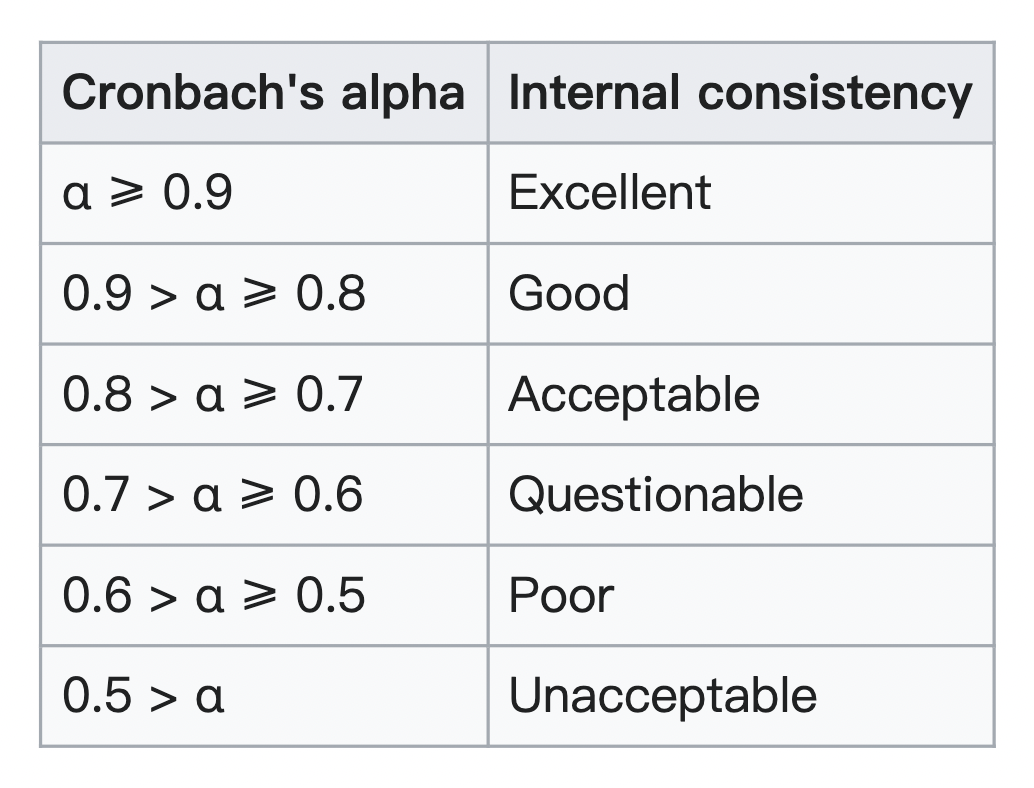
\includegraphics[width=0.5\linewidth]{Figure/Figure24.jpg}
  \centering
  \caption{Evaluation of score reliability coefficient test}
  \label{fig24}
\end{figure*}

\cleardoublepage
\subsection{SEM model 1}
\subsubsection{Path coefficient analysis}

SEM model 1 is shown in Figure~\ref{fig23}. The result of Regression Weights for Model 1 is shown in Table~\ref{table9}, and the result of Standard Regression Weights for Model 1 is shown in Table~\ref{table10}. From the result, we can find that Disaster Prevention Consciousness, Knowledge and Perception on earthquakes and Training Experience could show significant relationships with respondents' attitude toward Safety Tips, as p values are all less than 0.001. Also, Knowledge and Perception on earthquakes could show a positive relationship with respondents' attitude toward Safety Tips, as the estimated values are positive numbers (estimate value of Knowledge=3.066). While, Disaster Prevention Consciousness and Training Experience could show a negative relationship with respondents' attitude toward Safety Tips, as the estimate values are negative number (estimate value of Consciousness$=-2.191$; estimate value of Training Experience$=-0.433$;) 

\begin{figure*}[h]
  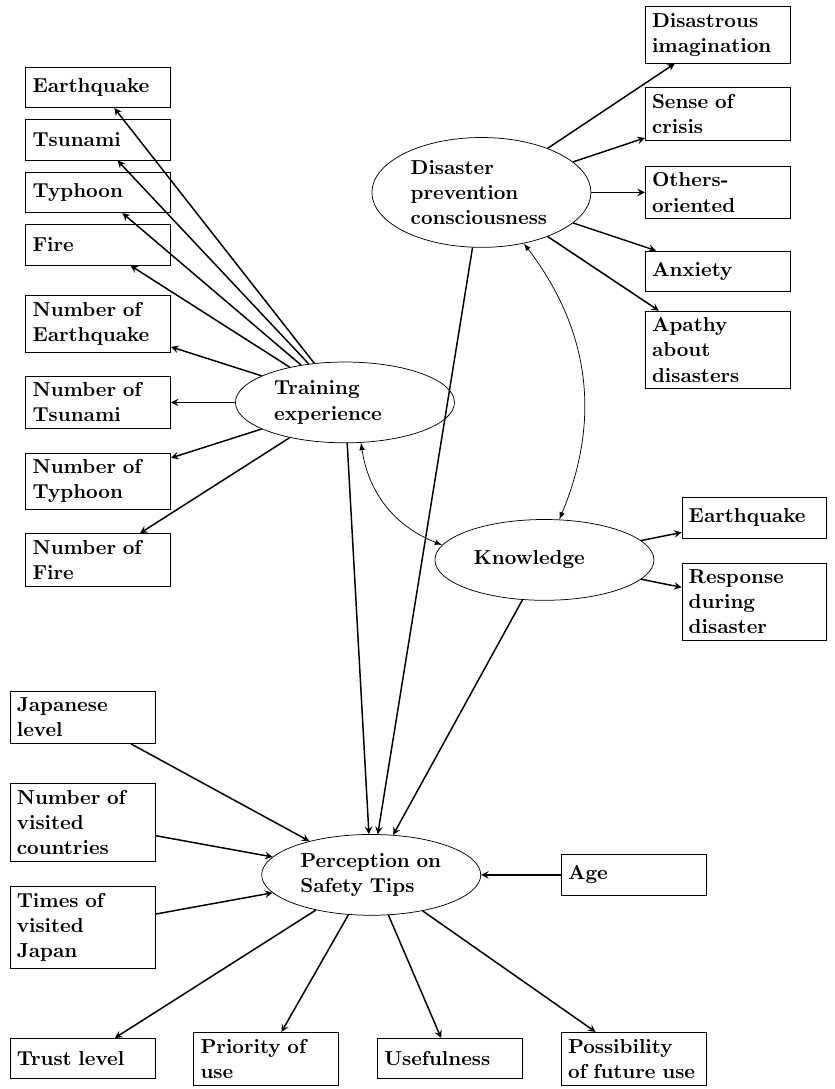
\includegraphics[width=0.5\linewidth]{Figure/Figure23.png}
  \centering
  \caption{SEM model 1}
  \label{fig23}
\end{figure*}

For four manifest variables, age, number of visited Japan, number of visited countries, and Japanese level don't show significant relationships with respondents' attitudes toward Safety Tips, as p values are larger than 0.01 ($p_{age} =0.633$; $p_{visitedJapan} =0.071$; $p_{visitedcountries} =0.628$; $p_{JapaneseLevel} =0.265$). 

\begin{table}[h]
  \caption{Regression Weights of SEM model 1 }
  \label{table9}
  \centering
  \begin{tabular}{lcl|c|c}
 \hline
 \multicolumn{3}{c|}{Regression Weights} & Estimate & p-value \\
 \hline
SafetyTips              &$\longleftarrow$ & age                  & 0.013  & 0.633                \\
SafetyTips              &$\longleftarrow$ & Training\_Experience & -0.501 & ***                  \\
SafetyTips              &$\longleftarrow$ & Consciousness        & -2.785 & ***                  \\
SafetyTips              &$\longleftarrow$ & Knowledge            & 4.336  & ***                  \\
SafetyTips              &$\longleftarrow$ & VisitCountry         & -0.012 & 0.628                \\
SafetyTips              &$\longleftarrow$ & Japanese\_Level      & -0.049 & 0.265                \\
SafetyTips              &$\longleftarrow$ & VisitJapan           & 0.041  & 0.071              \\
Q1\_disastrous\_imagination    &$\longleftarrow$ & Consciousness        & 1      &  \\
Q2\_ sense\_of\_crisis                      &$\longleftarrow$ & Consciousness        & 1.028  & ***                  \\
Q3\_others-oriented\_type                      &$\longleftarrow$ & Consciousness        & 1.029  & ***                  \\
Q4\_anxiety                      &$\longleftarrow$ & Consciousness        & 0.72   & ***                  \\
Q5\_ apathy\_about\_disasters                      &$\longleftarrow$ & Consciousness        & 0.157  & 0.052                \\
Q6\_1\_earthquake       &$\longleftarrow$ & Training\_Experience & 3.234  & ***                  \\
Q6\_2\_tsunami          &$\longleftarrow$ & Training\_Experience & 3.070   & ***                  \\
Q6\_3\_typhoon          &$\longleftarrow$ & Training\_Experience & 3.178  & ***                  \\
Q6\_4\_fire             &$\longleftarrow$ & Training\_Experience & 3.388  & ***                  \\
Q7\_1\_earthquake       &$\longleftarrow$ & Training\_Experience & 0.685  & ***                  \\
Q7\_2\_tsunami          &$\longleftarrow$ & Training\_Experience & 0.682  & ***                  \\
Q7\_3\_typhoon          &$\longleftarrow$ & Training\_Experience & 0.777  & ***                  \\
Q7\_4\_fire             &$\longleftarrow$ & Training\_Experience & 1      & \\
Q17\_Safetytips\_trust &$\longleftarrow$ & SafetyTips           & 1      &  \\
Q17\_Safetytips\_priority &$\longleftarrow$ & SafetyTips           & 0.826  & ***                  \\
Q17\_Safetytips\_usefulness &$\longleftarrow$ & SafetyTips           & 0.786  & ***                  \\
Q17\_Safetytips\_future\_use &$\longleftarrow$ & SafetyTips           & 0.688  & ***                 \\
 \hline
\multicolumn{5}{l}{*** means significant correlation at $p<0.001$.}
  \end{tabular}
\end{table}

\begin{table}[h]
  \caption{Standardized Regression Weights of SEM model 1 }
  \label{table10}
  \centering
  \begin{tabular}{lcl|c}
 \hline
 \multicolumn{3}{c|}{Standardized Regression Weights} & Estimate  \\
 \hline
SafetyTips              &$\longleftarrow$ & age                  & 0.015  \\
SafetyTips              &$\longleftarrow$ & Training\_Experience & -0.433 \\
SafetyTips              &$\longleftarrow$ & Consciousness        & -2.191 \\
SafetyTips              &$\longleftarrow$ & Knowledge            & 3.066  \\
SafetyTips              &$\longleftarrow$ & VisitCountry         & -0.016 \\
SafetyTips              &$\longleftarrow$ & Japanese\_Level      & -0.036 \\
SafetyTips              &$\longleftarrow$ & VisitJapan           & 0.058  \\
Q1\_disastrous\_imagination                      &$\longleftarrow$ & Consciousness        & 0.809  \\
Q2\_ sense\_of\_crisis                      &$\longleftarrow$ & Consciousness        & 0.843  \\
Q3\_others-oriented\_type                      &$\longleftarrow$ & Consciousness        & 0.855  \\
Q4\_anxiety                      &$\longleftarrow$ & Consciousness        & 0.576  \\
Q5\_ apathy\_about\_disasters                      &$\longleftarrow$ & Consciousness        & 0.092  \\
Q6\_1\_earthquake       &$\longleftarrow$ & Training\_Experience & 0.786  \\
Q6\_2\_tsunami          &$\longleftarrow$ & Training\_Experience & 0.838  \\
Q6\_3\_typhoon          &$\longleftarrow$ & Training\_Experience & 0.842  \\
Q6\_4\_fire             &$\longleftarrow$ & Training\_Experience & 0.758  \\
Q7\_1\_earthquake       &$\longleftarrow$ & Training\_Experience & 0.388  \\
Q7\_2\_tsunami          &$\longleftarrow$ & Training\_Experience & 0.489  \\
Q7\_3\_typhoon          &$\longleftarrow$ & Training\_Experience & 0.548  \\
Q7\_4\_fire             &$\longleftarrow$ & Training\_Experience & 0.566  \\
Q9\_knowledge\_earthquake                      &$\longleftarrow$ & Knowledge            & 0.785  \\
Q10\_knowledge\_response                     &$\longleftarrow$ & Knowledge            & 0.804  \\
Q17\_Safetytips\_trust &$\longleftarrow$ & SafetyTips           & 0.816  \\
Q17\_Safetytips\_priority &$\longleftarrow$ & SafetyTips           & 0.822  \\
Q17\_Safetytips\_usefulness &$\longleftarrow$ & SafetyTips           & 0.834  \\
Q17\_Safetytips\_future\_use &$\longleftarrow$ & SafetyTips           & 0.717  \\
 \hline
  \end{tabular}
\end{table}

The result of the correlation relationship between Disaster Prevention Consciousness with Knowledge and Perception on earthquakes, also Knowledge and Perception on earthquakes with Training Experience was shown in Table~\ref{table13} and Table~\ref{table14}. The result confirmed that Disaster Prevention Consciousness with Knowledge and Perception on earthquakes, also Knowledge and Perception on earthquakes with Training Experience could both show a significant correlation, as p values are all less than 0.001. And both are positive correlations, as the estimated values are positive numbers (estimate the value of Consciousness and Knowledge=0.961; estimate the value of Training Experience and Knowledge=0.18;). Among them, Disaster Prevention Consciousness with Knowledge and Perception on earthquakes could show a higher correlation than Knowledge and Perception on earthquakes with Training Experience. 

\begin{table}[h]
  \caption{Covariances of SEM model 1}
  \label{table13}
  \centering
  \begin{tabular}{lcl|c|c}
  \hline
   \multicolumn{3}{c|}{Covariances} & Estimate & p-value \\
  \hline
  Consciousness & $\longleftrightarrow$ & Knowledge & 0.589 & *** \\
  Training\_Experience & $\longleftrightarrow$ & Knowledge & 0.121 & *** \\
  \hline
\multicolumn{5}{l}{*** means significant correlation at $p<0.001$.}
  \end{tabular}
\end{table}

\begin{table}[h]
  \caption{Correlations of SEM model 1}
  \label{table14}
  \centering
  \begin{tabular}{lcl|c}
  \hline
   \multicolumn{3}{c|}{Correlations} & Estimate \\
  \hline
  Consciousness & $\longleftrightarrow$ & Knowledge & 0.961 \\
  Training\_Experience & $\longleftrightarrow$ & Knowledge & 0.180 \\
  \hline
  \end{tabular}
\end{table}
\cleardoublepage
\subsubsection{Model Fit Test}
The model fit result of Model 1 is shown in Table~\ref{table15}. From the results, CMIN/DF equals 8.352, an indicator that reflects model variability RMSEA equals 0.122, and an indicator that reflects model similarity CFI equals 0.738. Referring to some of the criteria mentioned in subsection~\ref{step6}, we can find that the model fit test of model 1 is not up to standard. Therefore, we need to modify model 1.

\begin{table}[h]
  \caption{Model fit test for SEM model 1}
  \label{table15}
  \centering 
  \begin{tabular}{|c|}
  \hline
  RMSEA = 0.122 \\
  CFI = 0.738 \\
  CMIN/DF = 8.352 \\
  \hline
  \end{tabular}
\end{table}

\subsubsection{Model adjustment and modification}

We can get a better estimate of the true correlation by disattenuated the variables, and according to D. Streiner (2006)~\cite{Streiner2006BuildingAB}, two things happen when we add extra variables. First, the model's ability to account for more variance grows. Each new variable, on the other hand, enhances the error variance. As a result, the previous model will struggle to accommodate the additional data, which is a consequence of adding more variables to the model. 

We can see that Q6 1/2/3/4 and Q7 1/2/3/4 both have a significant relationship with Training Experience based on the results of Table~\ref{table9} Regression Weights. However, the estimated values of Q7 (Q7\_1=0.388; Q7\_2=0.489; Q7\_3=0.548; Q7\_4=0.566) are much lower than the estimated value of Q6 (Q6\_1=0.786; Q6\_2=0.838; Q6\_3=0.842; Q7\_4=0.758) , as seen in Table~\ref{table10} Standardized Regression Weights. This means that Q6 could be better than Q7 at expressing the latent variable Training Experience. The two manifest variables are similar in structure: Q6 is for the experience of a given event, and the total score is used as data, whereas Q7 is for the number of times. Because the similarity of the two variables causes a significant amount of inaccuracy in the expression of the latent variable, we'll delete Q7 and keep only Q6 as the manifest variable to express latent variable Training experience as a way to improve the model. 

Another point that could be improved in Q5. From the regression weights results presented in Table~\ref{table9}, we can find that the only manifest variable that does not significant is Q5, as the p-value of Q5 with Disaster Prevention Consciousness is $p=0.052>0.001$. This means that Q5 does not work well as a manifest variable for latent variables Disaster Prevention Consciousness. Therefore, model 2 will remove Q5 and use only Q1 to Q4 as the manifest variables.

Then, since the results show that manifest variables age, number of visited Japan, number of visited countries, and Japanese level have no significant relationship with Attitude toward Safety Tips, deleting these four variables could be also a way to improve the model. 
Based on the above three improvement ideas shown on the left side of Figure~\ref{fig25}, we construct Model 2 shown on the right side of Figure~\ref{fig25}.

\begin{figure*}[t]
  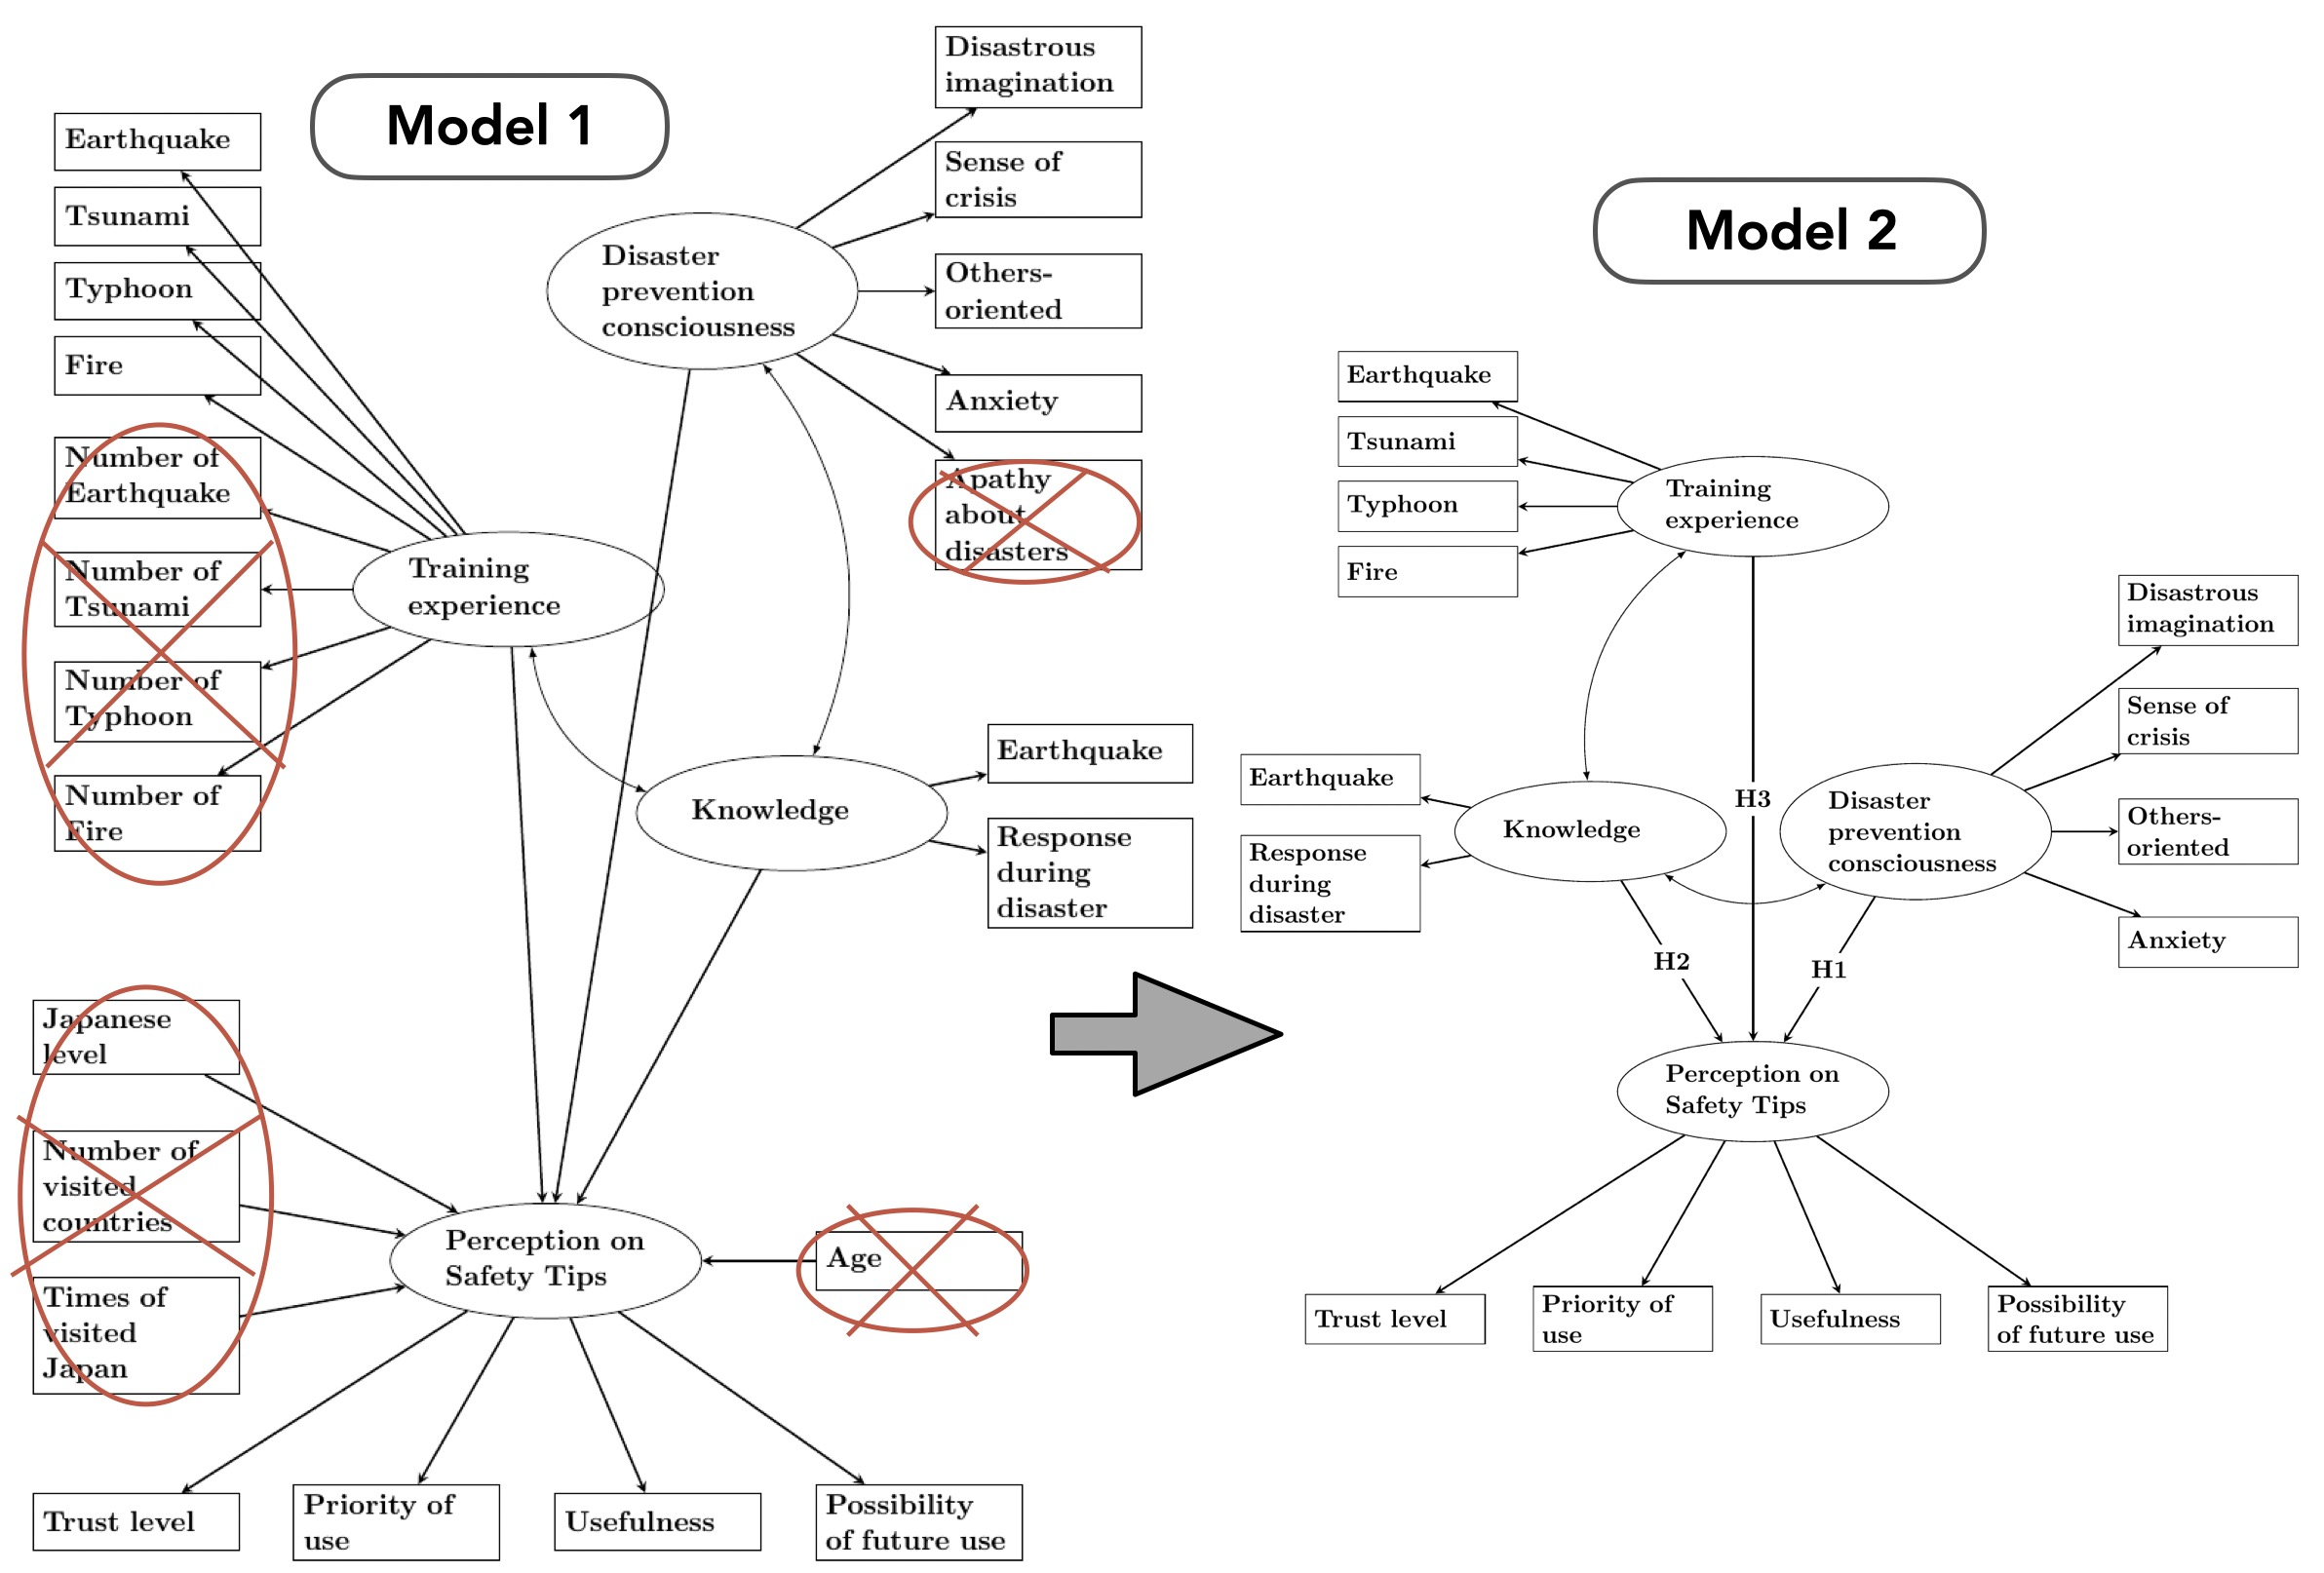
\includegraphics[width=\linewidth]{Figure/Figure25.png}
  \centering
  \caption[SEM model 2]{Left side: the diagram contains the improvement points made based on Model 1,Right side: Model 2}
  \label{fig25}
\end{figure*}


\subsection{SEM model 2}


\subsubsection{Model Fit Test}
The model fit result of model 2 is shown in Table~\ref{table16}. From the results, CMIN/DF equals 5.620, an indicator that reflects model variability RMSEA equals 0.097, an indicator that reflects model similarity CFI equals 0.925.

\begin{table}[h]
  \caption{Model fit test for SEM model 2}
  \label{table16}
  \centering 
  \begin{tabular}{|c|}
  \hline
  RMSEA = 0.097 \\
  CFI = 0.925 \\
  CMIN/DF = 5.620 \\
  \hline
  \end{tabular}
\end{table}

\subsubsection{Path coefficient analysis}
The result of Regression Weights for model 2 is shown in Table~\ref{table11}, and the result of Standard Regression Weights for model 2 is shown in Table~\ref{table12}. From the result, we can find that Disaster Prevention Consciousness, Training Experience, and Knowledge and Perception on earthquakes could show significant relationships with respondents' attitude toward Safety Tips, as p values are both less than 0.001. Then, from the result, we can find that Disaster Prevention Consciousness and Training Experience show opposite effects with Knowledge and Perception of earthquakes on respondents' attitude toward Safety Tips.  Disaster Prevention Consciousness and Training Experience could show a negative relationship with respondents' attitude toward Safety Tips, as the estimated values are negative numbers (estimate value of Consciousness=-2.253; estimate value of Training Experience=-0.414). Knowledge and Perception on earthquakes could show a positive relationship with respondents' attitude toward Safety Tips, as the estimated values are positive numbers (estimate value of Knowledge=3.127). Also, we can find that all manifest variables could significantly express latent variables, as the p-value of all manifest variables could be less than 0.001. 

\begin{table}[t]
  \caption{Regression Weights of SEM model 2 }
  \label{table11}
  \centering
  \begin{tabular}{lcl|c|c}
 \hline
 \multicolumn{3}{c|}{Regression Weights} & Estimate & p-value \\
 \hline
SafetyTips              &$\longleftarrow$ & Training\_Experience & -0.147 & 0.002**                \\
SafetyTips              &$\longleftarrow$ & Consciousness        & -2.876 & ***                  \\
SafetyTips              &$\longleftarrow$ & Knowledge            & 4.441  & ***                  \\
Q1\_disastrous\_imagination                      &$\longleftarrow$ & Consciousness        & 1      &  \\
Q2\_ sense\_of\_crisis                      &$\longleftarrow$ & Consciousness        & 1.027  & ***                  \\
Q3\_others-oriented\_type                      &$\longleftarrow$ & Consciousness        & 1.031  & ***                  \\
Q4\_anxiety                      &$\longleftarrow$ & Consciousness        & 0.715  & ***                  \\
Q6\_1\_earthquake       &$\longleftarrow$ & Training\_Experience & 1      &  \\
Q6\_2\_tsunami          &$\longleftarrow$ & Training\_Experience & 0.942  & ***                  \\
Q6\_3\_typhoon          &$\longleftarrow$ & Training\_Experience & 0.964  & ***                  \\
Q6\_4\_fire             &$\longleftarrow$ & Training\_Experience & 1.047  & ***                  \\
Q9\_knowledge\_earthquake                      &$\longleftarrow$ & Knowledge            & 1      &  \\
Q10\_knowledge\_response                     &$\longleftarrow$ & Knowledge            & 1.003  & ***                  \\
Q17\_Safetytips\_trust &$\longleftarrow$ & SafetyTips           & 1      &  \\
Q17\_Safetytips\_priority &$\longleftarrow$ & SafetyTips           & 0.827  & ***                  \\
Q17\_Safetytips\_usefulness &$\longleftarrow$ & SafetyTips           & 0.786  & ***                  \\
Q17\_Safetytips\_future\_use &$\longleftarrow$ & SafetyTips           & 0.688  & ***                 \\
 \hline
\multicolumn{5}{l}{*** means significant correlation at $p<0.001$.} \\
\multicolumn{5}{l}{** means significant correlation at $p<0.01$.}
  \end{tabular}
\end{table}

\begin{table}[h]
  \caption{Standardized Regression Weights of SEM model 2 }
  \label{table12}
  \centering
  \begin{tabular}{lcl|c}
 \hline
 \multicolumn{3}{c|}{Standardized Regression Weights} & Estimate  \\
 \hline
SafetyTips              &$\longleftarrow$ & Training\_Experience & -0.414 \\
SafetyTips              &$\longleftarrow$ & Consciousness        & -2.253 \\
SafetyTips              &$\longleftarrow$ & Knowledge            & 3.127  \\
Q1\_disastrous\_imagination                      &$\longleftarrow$ & Consciousness        & 0.809  \\
Q2\_ sense\_of\_crisis                      &$\longleftarrow$ & Consciousness        & 0.842  \\
Q3\_others-oriented\_type                      &$\longleftarrow$ & Consciousness        & 0.856  \\
Q4\_anxiety                      &$\longleftarrow$ & Consciousness        & 0.572  \\
Q6\_1\_earthquake       &$\longleftarrow$ & Training\_Experience & 0.792  \\
Q6\_2\_tsunami          &$\longleftarrow$ & Training\_Experience & 0.838  \\
Q6\_3\_typhoon          &$\longleftarrow$ & Training\_Experience & 0.833  \\
Q6\_4\_fire             &$\longleftarrow$ & Training\_Experience & 0.763  \\
Q9\_knowledge\_earthquake                      &$\longleftarrow$ & Knowledge            & 0.785  \\
Q10\_knowledge\_response                     &$\longleftarrow$ & Knowledge            & 0.804  \\
Q17\_Safetytips\_trust &$\longleftarrow$ & SafetyTips           & 0.817  \\
Q17\_Safetytips\_priority &$\longleftarrow$ & SafetyTips           & 0.824  \\
Q17\_Safetytips\_usefulness &$\longleftarrow$ & SafetyTips           & 0.835  \\
Q17\_Safetytips\_future\_use &$\longleftarrow$ & SafetyTips           & 0.718  \\
 \hline
  \end{tabular}
\end{table}

The result of the correlation relationship between Disaster Prevention Consciousness with Knowledge and Perception on earthquakes, also Knowledge and Perception on earthquakes with Training Experience was shown in Table~\ref{table21} and Table~\ref{table22}. The result confirmed that Disaster Prevention Consciousness with Knowledge and Perception on earthquakes, also Knowledge and Perception on earthquakes with Training Experience could still both show a significant correlation, as p-values are all less than 0.001. And both are positive correlations, as the estimated values are positive numbers (estimate the value of Consciousness and Knowledge=0.963; estimate the value of Training Experience and Knowledge=0.175;). Among them, Knowledge and Perception on earthquakes with Disaster Prevention Consciousness could show a higher correlation than it with Training Experience, which is as same as in SEM model 1.

\begin{table}[h]
  \caption{Covariances of SEM model 2}
  \label{table21}
  \centering
  \begin{tabular}{lcl|c|c}
  \hline
   \multicolumn{3}{c|}{Covariances} & Estimate & p-value \\
  \hline
  Consciousness & $\longleftrightarrow$ & Knowledge & 0.590 & *** \\
  Training\_Experience & $\longleftrightarrow$ & Knowledge & 0.383 & *** \\
  \hline
\multicolumn{5}{l}{*** means significant correlation at $p<0.001$.}
  \end{tabular}
\end{table}

\begin{table}[h]
  \caption{Correlations of SEM model 2}
  \label{table22}
  \centering
  \begin{tabular}{lcl|c}
  \hline
   \multicolumn{3}{c|}{Correlations} & Estimate \\
  \hline
  Consciousness & $\longleftrightarrow$ & Knowledge & 0.963 \\
  Training\_Experience & $\longleftrightarrow$ & Knowledge & 0.175 \\
  \hline
  \end{tabular}
\end{table}
\cleardoublepage
\subsubsection{Confirmatory Factor Analysis (CFA)}
CFA include Construct Validity, Convergent Validity and Discriminant Validity, as explained in subsection~\ref{step5}.

\textbf{Construct Validity.} Referring to some of the criteria mentioned in subsection~\ref{step6}, from the model fit test From the model fit result shown in Table~\ref{table16}, we can find that the CFI estimate is satisfied in model 2, as a CFI of 0.9 or higher can be considered a good match~\cite{ref43,ref44}. And according to Schumacker and Lomax (2004)~\cite{ref39}, they suggested a more lenient fit around 5 or less, and the current CMIN/DF is near to 5, but a little bit higher than 5. Finally for RMSEA, according to Takahiro HOSHINO (2005)  (SEMres), as current RMSEA$=0.097<0.1$, the model shows a moderate fit. For measuring model Disaster Prevention Consciousness shown in Figure~\ref{fig31}, the results of Standardized Regression Weights (SRW) and Squared Multiple Correlations (SMC) are shown in Table~\ref{table24} and Table~\ref{table25}. From the results, we can find that all the SRW values are greater than 0.55, which means that SMC is greater than 0.30, satisfying the criteria mentioned in subsection~\ref{s7}, proving good. The model fit result of measuring model Disaster Prevention Consciousness is shown in Table~\ref{table26}. From the results, we can find that all model fit estimates are highly satisfying the criteria mentioned in subsection~\ref{step6}, as CMIN/DF equals 2.963, RMSEA equals 0.063, CFI equals 0.996. 


\begin{figure*}[t]
  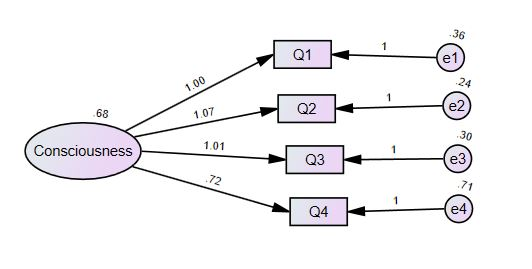
\includegraphics[width=0.5\linewidth]{Figure/figure31.JPG}
  \centering
  \caption{Measuring model of Consciousness}
  \label{fig31}
\end{figure*}

\begin{table}[h]
  \caption{Standardized Regression Weights for measuring model Consiousness}
  \label{table24}
  \centering
  \begin{tabular}{lcl|c}
  \hline
   \multicolumn{3}{c|}{Standardized Regression Weights} & Estimate \\
  \hline
  Q1 & $\longleftarrow$ & Consciousness & 0.807 \\
  Q2 & $\longleftarrow$ & Consciousness & 0.872 \\
  Q3 & $\longleftarrow$ & Consciousness & 0.835 \\
  Q4 & $\longleftarrow$ & Consciousness & 0.574 \\
  \hline
  \end{tabular}
\end{table}

\begin{table}[h]
  \caption{Squared Multiple Correlations for Consciousness}
  \label{table25}
  \centering
  \begin{tabular}{c|c}
  \hline
   Squared Multiple Correlations & Estimate \\
  \hline
  Q1  & 0.652 \\
  Q2  & 0.760 \\
  Q3  & 0.698 \\
  Q4  & 0.330 \\
  \hline
  \end{tabular}
\end{table}

\begin{table}[h]
  \caption{Model fit test for measuring model Consciousness}
  \label{table26}
  \centering 
  \begin{tabular}{|c|}
  \hline
  RMSEA = 0.063 \\
  CFI = 0.996 \\
  CMIN/DF = 2.963 \\
  \hline
  \end{tabular}
\end{table}

\textbf{Convergent Validity.} As mentioned in subsection~\ref{step5}, the commonly acceptable evaluation criterion of CR value in research should be above 0.7~\cite{ref32}. The result of the CR calculation is shown in Table~\ref{table35}. From the result, we can know that CR\_Consciousness$=0.857>0.7$; CR\_Training\_Experience$=0.882>0.7$; CR\_Knowledge$=1.001>0.7$; CR\_Attitude$=0.876>0.7$; This CR result can prove that the internal consistency of SEM is good. Also, according to Fornell and Larcker (1981)~\cite{ref31}, the commonly acceptable evaluation criterion of AVE value in research needs to be greater than 0.5. The result of the AVE calculation is also shown in Table~\ref{table35}. From the result, we can know that AVE\_Consciousness$=0.606>0.5$; AVE\_Training\_Experience$=0.651>0.5$; AVE\_Knowledge$=1.003>0.5$; AVE\_Attitude$=0.640>0.5$; This AVE result can prove that the explanatory power of the latent variables on the observed variables is good. In summary, the CR result and the AVE result show that SEM model 2 passed the Convergent Validity test. 

\begin{table}[h]
  \caption{Convergent Validity}
  \label{table35}
  \centering
  \begin{tabular}{lcl|cc|ccc}
  \hline
   & & & std.   & p-value           & SMC                  & CR                     & AVE                    \\
\hline
SafetyTips           & $\longleftarrow$       & Training\_Experience & -0.414 & 0.002                & \multicolumn{3}{l}{}    \\
SafetyTips           & $\longleftarrow$       & Consciousness        & -2.253 & ***                  & \multicolumn{3}{l}{} \\
SafetyTips           & $\longleftarrow$       & Knowledge            & 3.127  & ***                  & \multicolumn{3}{l}{}   \\
\hline
Q1                   & $\longleftarrow$       & Consciousness        & 0.809  &  & 0.654                & \multirow{4}{*}{0.857} & \multirow{4}{*}{0.606} \\
Q2                   & $\longleftarrow$       & Consciousness        & 0.842  & ***                  & 0.709                &                        &                        \\
Q3                   & $\longleftarrow$       & Consciousness        & 0.856  & ***                  & 0.733                &                        &                        \\
Q4                   & $\longleftarrow$       & Consciousness        & 0.572  & ***                  & 0.327                &                        &                        \\
\hline
Q6\_1                & $\longleftarrow$       & Training\_Experience & 0.792  &  & 0.627                & \multirow{4}{*}{0.882} & \multirow{4}{*}{0.651} \\
Q6\_2                & $\longleftarrow$       & Training\_Experience & 0.838  & ***                  & 0.702                &                        &                        \\
Q6\_3                & $\longleftarrow$       & Training\_Experience & 0.833  & ***                  & 0.694                &                        &                        \\
Q6\_4                & $\longleftarrow$       & Training\_Experience & 0.763  & ***                  & 0.582                &                        &                        \\
\hline
Q9                   & $\longleftarrow$       & Knowledge            & 0.785  &  & 0.616                & \multirow{2}{*}{1.001} & \multirow{2}{*}{1.003} \\
Q10                  & $\longleftarrow$       & Knowledge            & 0.804  & ***                  & 0.646                &                        &                        \\
\hline
Q17\_1               & $\longleftarrow$       & SafetyTips           & 0.817  &  & 0.667                & \multirow{4}{*}{0.876} & \multirow{4}{*}{0.64}  \\
Q17\_2               & $\longleftarrow$       & SafetyTips           & 0.824  & ***                  & 0.679                &                        &                        \\
Q17\_3               & $\longleftarrow$       & SafetyTips           & 0.835  & ***                  & 0.697                &                        &                        \\
Q17\_4               & $\longleftarrow$       & SafetyTips           & 0.718  & ***                  & 0.516                &                        &                       \\
  \hline
\multicolumn{5}{l}{*** means significant correlation at $p<0.001$.}
  \end{tabular}
\end{table}




\textbf{Discriminant Validity.} As mentioned in subsection~\ref{step5}, this study decided to use AVE to compare whether the mean AVE of two latent variables was greater than the squared correlation coefficient of the two latent variables~\cite{ref31} as the method of doing a Discriminant Validity test. Here, for operational convenience, we compare the positive square root of the AVE value of the latent variables and the correlation coefficient of the latent variables. The result of the calculation is shown in Table~\ref{table36}. From the result, we can find that SQRT\_AVE\_Knowledge=1.001, this value is larger than the correlation coefficient of Knowledge with the other three latent variables. Then, SQRT\_AVE\_Consciousness=0.778, this value is larger than the correlation coefficient of Consciousness with Training experience and Attitude, but it is smaller than the correlation coefficient of Consciousness with Knowledge. Next is SQRT\_AVE\_Training\_experience=0.807, this value is larger than the correlation coefficient of Training experience with the other three latent variables. Finally, SQRT\_AVE\_Attitude=0.800, this value is larger than the correlation coefficient of Attitude with Training experience and Consciousness, but it is smaller than the correlation coefficient of Attitude with Knowledge. As Discriminant Validity is to see whether the differentiation between different dimensions and between topics meets the standard. All the problematic items appear on top of Knowledge and Perception on earthquakes, which I think is due to the fact that there are only two manifest variables of this latent variable, which are not enough to accurately represent Knowledge and Perception on earthquakes on the SEM model. This is also a reason that the model fitness is affected in this study due to the limitation of survey data. But in general, the Discriminant Validity of this SEM model 2 could still be fine.

\begin{table}[h]
  \caption{Discriminant Validity }
  \label{table36}
  \centering
\makebox[1 \textwidth][c]{  
\resizebox{1\textwidth}{!}{
\begin{tabular}{c|ccccc}
\hline
     & AVE   & Knowledge                             & Consciousness                         & Training\_Experience                  & \multicolumn{1}{c}{SafetyTips}                          \\
\hline
Knowledge            & 1.003 & \textcolor{red}{\textbf{1.001}} & \multicolumn{1}{l}{}                  & \multicolumn{1}{l}{}                  &                                                         \\
Consciousness        & 0.606 & 0.963***                              & \textcolor{red}{\textbf{0.778}} & \multicolumn{1}{l}{}                  &                                                         \\
Training\_Experience & 0.651 & 0.175***                              & 0                                     & \textcolor{red}{\textbf{0.807}} &                                                         \\
SafetyTips           & 0.64  & 0.885***                              & 0.760***                              & 0.133                                     & \textcolor{red}{\textbf{0.8}}\\
  \hline
\multicolumn{5}{l}{*** means significant correlation at $p<0.001$.}
  \end{tabular}
}}
\end{table}

\subsubsection{Hypothesis testing and conclusion analysis}
\begin{itemize}
\item[\textbf{H1}] Disaster Prevention Consciousness has a positive impact on respondents' attitudes toward Safety Tips.
\item[\textbf{$\longrightarrow$}] This Hypothesis is inconsistent with hypothesis H1. Disaster Prevention Consciousness has a negative effect on respondents' attitudes toward Safety Tips.
\item[\textbf{H2}] Knowledge and Perception of earthquakes have a positive effect on respondents' attitudes toward Safety Tips.
\item[\textbf{$\longrightarrow$}] This Hypothesis is consistent with hypothesis H2. 
\item[\textbf{H3}] Training Experience has a positive effect on respondents' attitudes toward Safety Tips.
\item[\textbf{$\longrightarrow$}] This Hypothesis is inconsistent with hypothesis H3. Training Experience has a negative effect on respondents' attitudes toward Safety Tips.
\end{itemize}

\subsubsection{Interpretation}
The following sections will explain how to interpret the aforesaid results. 

Disaster Prevention Consciousness has a negative effect on respondents' attitudes toward Safety Tips: for all those who have a higher consciousness about the disaster, it means they have a higher disaster imagination, sense, and are more likely to feel anxiety about the disaster, and they are more likely to come into contact with people, so they would prefer a more direct way to evacuate rather than seeking information, which makes their attitude toward safety tips could be negative.
Knowledge and Perception of earthquakes have a positive impact on respondents' attitudes toward Safety Tips: people with richer knowledge, are relatively more aware of the importance of information seeking for evacuation. Therefore, their attitudes towards Safety Tips could be better than others.

Training Experience does not have a significant impact on respondents' attitudes toward Safety Tips: respondents with more earthquake or disaster training experience should be more knowledgeable with earthquake evacuation ways, therefore their attitude toward safety suggestions may be negative as well. 

Training Experience has a negative impact on respondents' attitudes toward Safety Tips: respondents with more earthquake or disaster training experience should be more knowledgeable with earthquake evacuation ways, therefore their response actions can separate from using applications on the cell phone. Therefore, their attitude toward safety suggestions may be negative as well. 













































